\documentclass{article}
\usepackage[dblblindworkshop]{neurips_2026}
\workshoptitle{TongNa Workshop}
\usepackage[utf8]{inputenc}
\usepackage[T1]{fontenc}
\usepackage{url}
\usepackage{booktabs}
\usepackage{amsfonts,amsmath,amssymb}
\usepackage{microtype}
\usepackage{graphicx}
\usepackage{multirow,array,multicol,adjustbox}
\usepackage{enumitem}
\usepackage{xcolor}
\definecolor{brandaccent}{RGB}{24,119,242}
\usepackage{xspace}
\usepackage{tikz}
\usetikzlibrary{arrows.meta}
\usepackage{algorithm}
\usepackage{algpseudocode}
\setlength{\emergencystretch}{3em}
% ===========================================================================
% numbers.tex -- every quantitative claim in the paper, defined in one place.
%
% The body never writes a literal number. It writes \val{key}, and the value
% lives here. Two reasons: a number that appears in the abstract, a table, and
% the discussion can only disagree with itself if it is typed three times; and
% a provisional number has to be visibly provisional until it is measured.
%
%   \defval{key}{value}   a measured number. Prints plain.
%   \defTBD{key}{guess}   not measured yet. Prints in accent bold while
%                         \hldraft is on, so it cannot ship unnoticed, and is
%                         listed by \printTBD.
%   \val{key}             use a number. An undefined key prints a red marker
%                         and raises a LaTeX warning rather than failing quietly.
%   \todo{note}           a prose-level gap, same visibility rules.
%   \printTBD             renders the outstanding-measurement list. Put it at
%                         the end of the document; it disappears with \hldraft.
%
% Camera-ready: \togglefalse{hldraft}. Every placeholder then prints as if it
% were real, which is exactly why \printTBD must read empty before that switch
% is thrown.
% ===========================================================================

\newtoggle{hldraft}
\toggletrue{hldraft}

\newcommand{\hlnumtbdlist}{}

\newcommand{\defval}[2]{\csdef{hlnum@#1}{#2}\csundef{hlntbd@#1}}
\newcommand{\defTBD}[2]{%
  \csdef{hlnum@#1}{#2}\csdef{hlntbd@#1}{}\listadd{\hlnumtbdlist}{#1}}

\newcommand{\val}[1]{%
  \ifcsdef{hlnum@#1}{%
    \ifcsdef{hlntbd@#1}{%
      \iftoggle{hldraft}{\textcolor{brandaccent}{\bfseries\csuse{hlnum@#1}}}%
                        {\csuse{hlnum@#1}}%
    }{\csuse{hlnum@#1}}%
  }{%
    \textcolor{red}{\bfseries[?\,\texttt{#1}]}%
    \PackageWarning{hlnumbers}{Undefined number key '#1'}%
  }%
}

\newcommand{\todo}[1]{%
  \iftoggle{hldraft}{\textcolor{red}{\bfseries[TODO: #1]}}{}}

\newcommand{\hlnumtbditem}[1]{\item \texttt{#1} \dotfill\ \csuse{hlnum@#1}}
\newcommand{\printTBD}{%
  \iftoggle{hldraft}{%
    \section*{Outstanding measurements}
    Placeholders still standing in for unmeasured quantities. This list must be
    empty before submission.
    \begin{itemize}[nosep,leftmargin=*]
      \forlistloop{\hlnumtbditem}{\hlnumtbdlist}
    \end{itemize}}{}}

% ---------------------------------------------------------------------------
% Archive scale. Editions and founding year are documented facts; the
% submission and match counts were quoted as round approximations in the
% proposal and need an exact recount off the archive before they are claims.
% ---------------------------------------------------------------------------
% Keys hold bare quantities, never connective words: "X of nine" or "XXth" bakes
% English grammar into the value and cannot be reused by the Chinese abstract.
% Connectives live in the prose. Two values are unavoidably prose (loseaxis,
% ceilingcause) and carry a *zh sibling.
% 1997 was the first edition, so 2026 is the 30th. The proposal's "27 editions"
% counted through 2023.
\defval{editions}{30}
\defval{founded}{1997}
\defTBD{nsub}{$\sim$10{,}000}
\defTBD{nmatch}{$\sim$100{,}000}
\defval{ngames}{9}

% ---------------------------------------------------------------------------
% The audit: does the folk hierarchy predict who wins? Descriptive shares over
% the archive, no counterfactual claimed. The RL scarcity here is confounded by
% student cost structure -- addressed in the introduction, not the abstract.
% ---------------------------------------------------------------------------
\defTBD{pheur}{XX\%}
\defTBD{prl}{X.X\%}
\defTBD{nrlfinal}{X}

% ---------------------------------------------------------------------------
% Headline result. Percentile of the human field is the metric the archive
% uniquely affords: a skill gradient rather than one reference solution.
% ---------------------------------------------------------------------------
\defTBD{pct}{XX}
\defTBD{nbeat}{X}
\defTBD{elogap}{$+$XX}

% ---------------------------------------------------------------------------
% Sample efficiency against RL. The crossover matters more than the ratio: the
% claim is budget-conditional, not a claim that HL dominates. loseaxis names
% the denominator on which HL is the worse method, stated up front on purpose.
% ---------------------------------------------------------------------------
\defTBD{effratio}{XX$\times$}
\defTBD{crossover}{$\sim$XXX k}
\defTBD{loseaxis}{per wall-clock hour and per dollar}

% ---------------------------------------------------------------------------
% The ceiling. Frontier-Eng (arXiv 2604.12290) reports improvement frequency
% decaying as t^-1 with a plateau by 50-100 iterations on single-agent tasks.
% Whether an adversarial setting decays slower is the interesting comparison,
% so the exponent is a measured quantity here, not an assumed one.
% ---------------------------------------------------------------------------
\defTBD{decay}{$t^{-\alpha}$}
\defTBD{plateau}{$\sim$XX}
% Prose-valued keys stay English-only: the document is compiled with pdfLaTeX,
% which cannot typeset CJK without CJKutf8, and \printTBD renders every
% registered key whether the body cites it or not.
\defTBD{ceilingcause}{TBD mechanism}
\defTBD{ntransfer}{X}

\newcommand{\benchname}{\mbox{HL-Arena}\xspace}

\title{How Far Can Heuristic Learning Go in Adversarial Games?\\
Characterizing Performance Ceilings, Complexity, and Sample Efficiency
against a Real-World Human Field}
\author{Anonymous Submission}

\begin{document}
\maketitle
\begin{abstract}
We study heuristic learning (HL) in adversarial games: a coding agent reads
environment feedback and directly revises a persistent, executable heuristic
policy while the base model remains frozen. Unlike prompt optimization or
population-based search, each round edits the single artifact produced by the
previous round. We evaluate this setting on \benchname, an archive-backed suite
of adversarial games with human-written programs, and compare it with learned
reinforcement-learning policies under matched interaction budgets. Our protocol
measures performance against the human field, sample efficiency, and the
maintenance capacity at which policy revisions cease to pay. The resulting
comparison makes explicit when an editable program is a useful learning object
and when a learned policy is the better use of interaction budget.
\end{abstract}

% ---------------------------------------------------------------------------
% Introduction
%
% The chain, in order. Each link is one paragraph and each exists to make the
% next one necessary:
%
%   1. RL's home turf is adversarial games -- so the comparison happens where
%      RL is strongest, not where it is weakest.
%   2. Concede the extensibility objection, then relocate it: it describes the
%      author, not the artifact.
%   3. Coding agents change who the author is. The operative property is
%      editability, not interpretability.
%   4. The question, announced as two-sided.
%   5. Lower bound: information per sample. The on-policy/off-policy spectrum,
%      cross-policy-class data reuse, rules as a non-sample prior. The spectrum
%      is also the reason model-based RL has to be the primary baseline: against
%      policy gradient alone, symbolic-vs-neural is confounded with
%      on-policy-vs-off-policy. Keep that sentence attached to this link -- it
%      reads as an unmotivated methods note anywhere else.
%      This link ends by giving away more than it looks like: the
%      information-per-sample gain is NOT the symbolic form's doing, since a
%      memory-based agent holding no program gets it too (echo2025hindsight).
%      Conceding that is what keeps the two bounds independent, which is the
%      whole structure of the paper -- the lower bound is about what the loop
%      can read, the upper about what it can edit, and only the second is the
%      program's. Deleting the concession to strengthen the lower bound would
%      collapse them into one claim and hand a referee the objection ("then why
%      the program at all?") with no answer in the text.
%      Keep the system NAMES in both places -- "ECHO" here and "DiPRL" in the
%      editability paragraph. Chengpeng Hu (diprl2026) and Michael Y. Hu
%      (echo2025hindsight) are different people, and natbib renders both as
%      "Hu et al." with only the year to tell them apart, so the two read as one
%      group's pair. Naming the systems is what disambiguates them for a reader;
%      do not revert either to "a recent system". Found by reading the rendered
%      intro end to end -- no mechanical check catches it.
%   6. Upper bound, in four paragraphs: the mechanism (accumulation defeats
%      placement); the external evidence for it (SlopCodeBench); the two results
%      isolating the mechanisms underneath, which are about context and
%      execution rather than code quality (longcontextbugfix2026,
%      longhorizonexecution2026); and the distinction that keeps our loop
%      tractable (their spec grows, a game's rules do not, so a heuristic can be
%      replaced rather than layered). This was three paragraphs until the
%      citation check expanded the evidence; do not merge them back, the
%      combined version ran twenty rendered lines and carried three papers.
%      All three citations were verified against full text 2026-08-18 and all
%      three needed correction -- see their refs.bib annotations, which are
%      authoritative, and note in particular that longhorizonexecution2026's
%      own thesis runs opposite to the use we make of it.
%      Two claims about SlopCodeBench were drafted wrong and are now fixed
%      against the v2 full text; both flattered us, which is why they lasted.
%      (a) Human repos do NOT "flatten". 68% of them end more verbose than they
%      began. The finding is a rate gap -- per-checkpoint slope 0.0022 vs 0.0144
%      for verbosity -- and the rate gap is the better claim anyway, since a
%      human exemption would make maintenance capacity look like an
%      agent-specific defect instead of a general limit that agents hit sooner.
%      (b) Never write that quality-aware prompting leaves the slope
%      "statistically unchanged". Their paper runs no significance test on that
%      experiment at all; "slope" and "intercept" appear only in Appendix D,
%      about the human panel. Say the prompts move the starting level without
%      slowing the growth -- and keep the price attached (2.3 pp of strict
%      correctness, 12.1% cost), because an intervention that trades capability
%      for initial quality and still does not bend the curve is the actual
%      argument for a capacity limit. All figures live in the refs.bib
%      annotation, which is authoritative; re-verify if a v3 appears, since
%      every v1 number changed in v2 and this paragraph inherited the v1 set.
%      Then the axis: description length of a good-enough policy against the
%      agent's maintenance capacity. Go is the counterexample that kills rule
%      complexity as the x-axis. The LLM boundary falls out of the same axis.
%      The inequality must state its observable signature where it is introduced
%      -- convergent stall size across games, divergent Elo at that size -- and
%      must say that it is the PAIR that does the diagnosing. Until 2026-08-18
%      this paragraph called the plateau "diagnostic" without saying how it could
%      be observed, and the signature appeared only in the contributions, which
%      asserted the result with no mechanism attached. Convergent length alone
%      proves nothing: it is equally consistent with games that never differed in
%      complexity.
%   7. Why the question is still open. The heading said "Why this ceiling has not
%      been measured" until 2026-08-18, which is this link's own prohibition
%      stated at heading level, and which its first clause then contradicted.
%      Headings get written early and revised least: check them against these
%      notes separately from the body. Careful: agent self-improvement
%      decay HAS been measured (frontiereng2026 -- frequency t^-1 AND magnitude
%      k^-1, marginal returns near zero after ~50-100 iterations, tail to 500).
%      Do not compress this to "plateau within tens of iterations", which the
%      paragraph said until 2026-08-18: it is the wrong number and the wrong
%      shape. Cite both exponents. Do not write "never measured" -- concede the
%      result and say what it lacks: single-agent tasks, no human field, no RL
%      baseline. The
%      confound we remove is a different one, human iteration cost.
%   8. The venue.
%   9. HL, plus the selection-effect concession.
%  10. Contributions.
%
% Four things to hold onto while editing:
%   - The objection is conceded, never refuted. "Everyone was wrong" is both
%     weaker and less true than "everyone was measuring the author".
%   - Paragraphs 5 and 6 stay adjacent. Split them and the paper reads as two
%     unrelated findings instead of one bound with two sides.
%   - Do not write "if-else". Characterizing what the winning programs contain
%     is a result, not a punchline.
%   - Do not claim editability as our coinage. Programmatic RL already calls
%     its policies human-editable; what changes here is the role the property
%     plays -- precondition for the optimizer, not feature of the deliverable.
%   - In paragraph 6, never let rule complexity back in as the axis. An earlier
%     draft rejected it with the Go example and then wrote "rule complexity and
%     revision count are the same axis seen twice" three sentences later, which
%     contradicts the paragraph's own thesis. The axis is K(pi_good), always.
%     A game defeats the loop because its *winning policy* is long, not because
%     its rulebook is.
%     Related, and also drafted wrong once: do not write that a hard game
%     "starts near the capacity". The program grows from a naive draft in every
%     game; the capacity is fixed by the agent. What varies across games is where
%     K(pi_good) sits relative to that ceiling -- below it, the program reaches
%     winning strength before it becomes unmaintainable; above it, the program
%     stops improving while still short of winning. Getting this backwards makes
%     the paper's central inequality read as though the game moved the ceiling.
%
% LENGTH. Roughly 2,200 words plus 400 of contributions, which is long. It is
% long because the argument is two-sided, carries external evidence, and answers
% two objections before the results -- all deliberate. Do not trim it to a target
% without a venue actually demanding one. When one does, cut in this order:
%   1. The editability discussion in para 3, from four sentences to two. The
%      distinction is needed; the elaboration is not.
%   2. The contamination-resistance contrast, to one sentence. It is positioning
%      against a literature, and the benchmark section makes the same case.
%   3. The two objection paragraphs, merged and moved to Limitations. This costs
%      real credibility -- a reader who meets the pretraining objection first in
%      Section 6 has already decided we were hiding it -- so it goes last.
% Never cut: the Go example (it is what kills rule complexity as the axis), the
% single inequality, or the replacement-vs-accumulation distinction.
% ---------------------------------------------------------------------------

\section{Introduction}

Reinforcement learning (RL) established itself on adversarial games. Chess, Go,
shogi, StarCraft, and Dota were where learned policies first beat the strongest
humans alive, and where the field's characteristic result took shape: a policy
trained by self-play, given enough interaction, exceeds anything a person wrote by
hand \citep{alphazero2018,alphastar2019,openaifive2019}. Games are also where the
symbolic alternative --- rules, an evaluation function, a search procedure --- was
judged to have the lower ceiling, and this paper stays on that turf rather than
retreating to a setting chosen to favour programs.

The objection is that a program exhibits only the behaviour somebody wrote down:
every new case has to be noticed, encoded, and reconciled with the rules already
present, at a cost that grows with the program. This is correct and we do not
dispute it. But it is a claim about the author, not the artifact. Nothing in the
symbolic paradigm caps what a program can express --- the cap is on how much of it
a human will maintain before the reconciliation cost exceeds what they can pay.
Asymptotically the learned policy still wins. The question is what happens under a
budget, where the authoring cost is the binding term.

\paragraph{What coding agents changed.} They change who the author is, and the
property that matters once the author is a machine is not the one usually
argued. The axis is \emph{editability}, not interpretability: interpretability
asks whether a human understands the policy, which a reader may reasonably not
care about, while editability asks whether the optimization loop can act on the
artifact at all. A symbolic program can be read in full and changed in part, and
takes the heterogeneous inputs maintenance requires --- rules, its own source,
replays of losses. A learned policy admits no comparable loop: its behaviour lives
in weights that cannot be edited locally and offer no handle by which a specific
failure traces to a specific parameter. The two properties do come apart --- a
system can reason in natural language about every decision it makes and still hold
its policy in weights \citep{tig2025think} --- and programmatic RL already calls
its policies human-readable and editable \citep[DiPRL;][]{diprl2026}. What changes
here is the role the property plays: not a feature of the delivered artifact, but
the reason an optimizer exists for it.

So the question reopens, and this time it is measurable: \emph{how far does the
symbolic paradigm go once a machine pays the maintenance cost?} The answer is
two-sided --- an agent-maintained program wins for a reason having nothing to do
with expressiveness, and stops for a reason having everything to do with the program
and nothing to do with the paradigm.

\paragraph{Why an agent-maintained program wins under a budget.} The binding
constraint under a budget is information per sample. A scalar reward reports that
an episode went badly; the rules plus a replay of the loss report what happened,
when the position turned, and which decision was responsible --- and the
difference compounds, because it determines how much of the sample survives to the
next revision. Policy-gradient methods are on-policy, using a batch for one update
and discarding it \citep{offpolicyvaluellm2026}; off-policy methods reuse it
\citep{samplereuse2022}. A maintained program sits at the far end of that
spectrum: off-policy and \emph{cross-policy-class}, able to learn from replays of
any opponent and from human source code no gradient method can consume, and it
reads the rules directly --- a prior obtained without spending samples at all. An
LLM revising a Python policy from execution traces is already competitive with
deep-RL baselines on single-agent tasks at far fewer environment interactions
\citep{kuang2025generative}, though only directionally: one family of tasks, no
shared budget accounting, no adversary. The spectrum also settles how the
comparison must be run, since measuring against policy gradient alone confounds
symbolic-versus-neural with on-policy-versus-off-policy --- so model-based RL is
our primary baseline and policy gradient the on-policy reference point.

The advantage is narrower than it looks, and the narrow version is the one worth
defending. ECHO rewrites its own failed episodes into usable experience and becomes
more sample-efficient holding no program at all \citep{echo2025hindsight}: what
buys the information per sample is the reader, not the symbolic form. The program
earns its place on the other side of the question, as what makes the policy an
object the loop can edit --- and therefore as what sets where the loop stops. The
two bounds are measured against different things: the lower against RL's sample
budget, the upper against the agent's own capacity.

\paragraph{Why it stops.} What the loop accumulates is what eventually stops it.
Revisions leave the program larger and more interconnected, and each further
revision has to place an edit without disturbing what already works; past some size
that placement fails more often than it succeeds --- not because the paradigm ran
out of expressiveness, but because the artifact outgrew what its maintainer can
hold, attribute, and change. This is measurable outside our setting. Coding agents
extending their own prior
code accumulate structural damage as they go, at rising cost and no matching gain
in correctness; human maintainers are not exempt but accumulate it several times
more slowly per revision, so what separates a maintainer that keeps working from
one that stalls is a rate rather than an exemption
\citep{slopcodebench2026}. Quality-aware prompting lowers the starting level
without slowing the growth, and costs correctness to do it --- the signature of a
capacity limit rather than a prompting defect. Two mechanisms underneath are not
about code quality at all: agentic repair succeeds only while the context each step
accumulates stays small, which locates the advantage in decomposition rather than
retrieval \citep{longcontextbugfix2026}; and given the plan up front, per-step
accuracy still falls as steps accumulate, models erring more once their own earlier
errors are in context \citep{longhorizonexecution2026}. Reasoning mitigates that
second failure, which helps us rather than hurts --- a plateau reached by a
reasoning agent cannot be attributed to self-conditioning --- and what survives is
the finite single-turn execution horizon each frontier model has, an order of
magnitude apart between them. That is capacity as a property of the agent rather
than of the task, and a program under revision is the case that cannot be
decomposed away: the artifact is the accumulated context, and every revision has to
hold it whole.

The evidence cuts both ways, though. Their decay is driven by a specification that
keeps growing, so nothing may be discarded; a game's rules do not change, so a
better heuristic may \emph{replace} a worse one instead of being layered on top of
it and the program is free to get shorter. Accumulation is a tendency here rather
than an obligation --- which is why the ceiling is worth measuring instead of
assuming, and why we log program size at every revision rather than only Elo.

The axis this limit falls on is a description length, and not the length of the
rules. Go's rules fit on a page, yet no compact symbolic policy plays it well ---
the programs that do carry their strength in weights --- while a contest game may
run to pages of special cases and still admit a strong policy in a few hundred
lines. What governs the outcome is the description length of a \emph{symbolic}
policy good enough to win, which we write $K(\pi_{\mathrm{good}})$ after
Kolmogorov complexity and estimate through a compression proxy, the quantity itself
being uncomputable \citep{lividanyi2019kolmogorov,rissanen1978mdl}. The prediction
is a single inequality: HL succeeds while $K(\pi_{\mathrm{good}})$ stays below the
agent's maintenance capacity, and plateaus as it approaches it. Since the program
grows from a naive draft in every game, what differs is where the target sits
relative to the ceiling --- below it, the program reaches winning strength before it
becomes unmaintainable; above it, the program stops improving while still short.
And because the capacity belongs to the agent, this predicts a signature: the size
at which the loop stalls should be roughly the same from game to game while the
strength reached there should not, and it is that pairing, not either half, that
distinguishes a limit of the maintainer from a limit of the game. The paradigm's
boundary then follows without a separate argument: tasks at the scale of language
modelling lie outside it not because they are adversarial or unstructured, but
because no policy of a maintainable description length is any good at them. And
since the ceiling belongs to the maintainer, it moves with model capability, which
is why it can be measured at all.

\paragraph{Why the question is still open.} Agent self-improvement is already
known to decay, and from both directions at once: across 47 real engineering
tasks, improvement frequency falls as $t^{-1}$ while the magnitude of the $k$-th
improvement falls as $k^{-1}$, a double squeeze driving marginal returns near zero
after 50 to 100 iterations \citep{frontiereng2026}. What that leaves open is where
the symbolic paradigm stands against a learned one, since those tasks are
single-agent and carry neither a human field nor an RL baseline. Where both
reference points were present, the maintainer was always human, so the paradigm
and the cost of human iteration were measured together: a heuristic program that
stopped improving might have exhausted the paradigm or exhausted its author's
weekend, and the record cannot say which. Replacing the author with an agent holds
the paradigm fixed and changes the cost of iteration --- the term that was never
varied.

\paragraph{Where to measure it.} The question needs a domain where many
independent authors pushed the symbolic paradigm as far as a real budget allowed,
with the results recorded and the budget the same for every method they might have
chosen. We use the complete archive of a collegiate game AI contest running since
\val{founded}: games authored for the contest itself, \val{nsub} submissions, and
\val{nmatch} adjudicated matches, written under deadline with standings at stake.
Contests of this kind carry a folk ordering of methods --- rules for beginners,
search for the intermediate, RL as the highest ceiling --- which is worth naming
because it is the ordering the field's own results are taken to endorse. The
archive records that this ordering gets the asymptotic ceilings right and still
fails to predict who wins: \val{pheur} of prize-winning programs contain no
learned component, and RL, present in \val{prl} of submissions, reached the finals
in \val{nrlfinal} of \val{editions} editions.

Two properties follow from provenance rather than design. Contamination resistance
is usually bought by authoring fresh tasks or collecting new ones continuously
\citep{livecodebench2024,workbuddybench2026}; here it comes from a venue that
predates the benchmark and was never built for evaluation --- which we still verify
rather than assume. And because thousands of people attempted the same games, the
archive carries a \emph{distribution} of human skill rather than a reference
solution, so a method can be placed at a percentile of a real field, as agents have
been placed against Kaggle competitors and informatics olympiad contestants
\citep{mlebench2024,olympiad2025percentile}.

\paragraph{Heuristic learning.} We remove the confound with heuristic learning
(HL): a coding agent maintains a heuristic program by reading the rules, its own
source, and replays of its losses, then rescores it against a frozen opponent pool.
The loop is deliberately narrow --- one revision per iteration, every version and
score kept --- because attribution is the property we are trying to preserve. Its
evaluator is a game engine and its opponents are frozen, placing it at the strong
end of the verification hierarchy along which demonstrated self-improvement tracks
\citep{selfimprovement2026survey}.

That this is not merely a matter of a stronger model matters, because the closest
existing head-to-head found the humans winning: across 38{,}304 matches,
human-written agents took the top five places and a frontier model handed the
winning student's program dropped it to tenth
\citep{vibecoding2025tournament}. Their agents were not one-shot --- most were
revised and all were debugged over many cycles --- but that loop optimized
compilability, and no agent was ever revised against the tournament it would be
judged in. The gap is therefore neither model capability nor a missing edit; it is
the absence of many revisions carrying an adversarial signal, which is the loop this
paper measures.

Two objections are conceded here and answered in full in
Section~\ref{sec:discussion}. The agent arrives with a pretraining corpus while RL
starts cold, and no denominator makes that symmetric; we report environment steps
as what is scarce in a new domain, and test what pretraining supplies
(Section~\ref{sec:experiments}) rather than asserting it. And the archive's RL
scarcity is confounded with its participants' cost structure --- students on a
deadline have limited compute, time, and RL expertise --- so what it records is
what wins under contest constraints, at one budget applied to whichever method a
contestant chose. Every comparison here is budget-conditional.

\subsection*{Contributions}

% Method, benchmark, comparison -- in that order, so the algorithm is the paper's
% subject and the benchmark is what it is measured on. The archive audit sits
% under the benchmark: it describes what the archive contains, and is not a
% result of comparing HL against RL.
\begin{itemize}[leftmargin=*]
  \item \textbf{Heuristic learning (HL): agent-maintained symbolic policies under
  adversarial pressure, instrumented so the ceiling can be located.} That an LLM
  can revise a program from execution feedback is established
  \citep{kuang2025generative}; what HL adds is the adversary and the discipline ---
  one revision per iteration, every version and score in an append-only log, so
  that a change in behaviour is attributable to the edit that caused it. Without
  that attribution a plateau can be observed but not diagnosed.

  \item \textbf{A benchmark drawn from a real competition rather than constructed
  for evaluation.} To the archive's \val{nsub} submissions and \val{nmatch}
  adjudicated matches --- written to win under deadline, not authored as tasks ---
  we add the apparatus a benchmark needs: classic games as structural controls,
  three opponent pools (training, frozen test, Elo anchor), a frozen evaluation
  set, and an Elo protocol comparable across games and editions. We also classify
  every submission by whether it contains a learned component, which is what makes
  the audit above a measurement rather than an impression.

  \item \textbf{A broad comparison of HL and RL, and a mechanism for where HL
  stops.} Against model-based RL, policy gradient, and the human field, over a
  range of budgets, reported in every denominator rather than the favourable one:
  HL reaches the \val{pct}th percentile of the field and beats the strongest
  recorded human on \val{nbeat} games, and is \val{effratio} more sample-efficient
  than model-based RL at matched Elo --- but that baseline overtakes beyond
  \val{crossover} environment steps and HL costs more \val{loseaxis}. Neither
  paradigm dominates; the budget and the game's structure decide. Improvement
  frequency decays as \val{decay} and plateaus near \val{plateau} revisions, which
  we trace to maintenance capacity on a pair of quantities: description length at
  the plateau converges to \val{maintcap} within \val{maintcapspread} across games
  of differing complexity, while the Elo reached there varies by
  \val{eloplatspread}. Equal maintainable size at unequal strength is what
  separates a limit of the agent from a limit of the game --- convergent length
  alone would not, being equally consistent with games that never differed. The
  loop transfers to \val{ntransfer} further benchmarks without retuning.
\end{itemize}


% ---------------------------------------------------------------------------
% Heuristic Learning
%
% RENAMED from "Methodology" on 2026-08-19 and split into two subsections at the
% user's direction: Motivation, then Introducing HL. The section now carries the
% DEFINITION, not just the loop.
%
% THE DEFINITION, in the user's own words (2026-08-19): heuristic learning is the
% paradigm of using an agent to understand feedback and directly modify a program
% or other interpretable system. Two things follow that the rest of the paper does
% not yet reflect:
%   - it is NOT game-specific. "Program or other interpretable system" is the
%     general object; adversarial games are the setting we measure it in, not the
%     definition's scope. The introduction currently frames HL game-specifically
%     ("a coding agent maintains a heuristic program ... rescores it against a
%     frozen opponent pool"), which is the instantiation. State the general form
%     here first, then narrow to the game instantiation explicitly, so a reader
%     cannot mistake the benchmark for the boundary of the paradigm.
%   - "understand feedback" and "directly modify" are the two halves, and they map
%     onto the two bounds the paper already argues: what the loop can READ (lower
%     bound, information per sample) and what it can EDIT (upper bound,
%     maintenance capacity). The definition is where those two are introduced as
%     one object; do not let the subsections split them apart.
%
% WRITTEN 2026-08-19: 3.1 (four paragraphs + Figure 1) and 3.2's opening (the
% definition, the two-agent loop, Figure 2, the two costly constraints). What is
% written is the user's own outline: expressiveness and interpretability, the size
% figure, the program space as a convenient destination for human experience, the
% maintenance cost, then the agent-era reversal (input and output space IS program
% text, so both halves of the loop run in one representation), then the loop itself.
%
% TWO JUDGEMENT CALLS in 3.1, both reversible:
%   - The user's phrasing was that HL is "a robust architecture with very high
%     information flow". The written version claims the information flow (that is
%     architectural and follows from the representation argument) but NOT the
%     robustness, which is \val{robustspread} and unmeasured. Calling the
%     architecture robust in the motivation is invariant 9 exactly -- the framing
%     ahead of the number -- and it would be the second time robustness got asserted
%     before it had a result behind it. When \val{robustspread} exists, this is where
%     the claim can be made if it holds.
%   - The maintenance paragraph was rewritten once because its first version
%     restated 01-introduction.tex's "every new case has to be noticed, encoded, and
%     reconciled ... at a cost that grows with the program" almost clause for clause.
%     What this section adds and the intro does not have: the cost is in the
%     CHECKING, not the writing, which is why it grows rather than staying flat. If
%     that distinction is ever cut, cut the paragraph -- without it the paragraph is
%     the intro again.
%
% STILL OWED BY THIS SECTION, none of it written yet: everything in the blocks
% below. The lower-bound argument, the on/off-policy spectrum (offpolicyvaluellm2026,
% samplereuse2022 -- still cited nowhere in body text), the echo2025hindsight
% concession in its empirical form, the description-length protocol, the baseline
% rationale, the budget-commensurability conversion, and the measurement definitions.
% 3.2 currently stops after the loop; the protocol half of it is absent.
%
% MOTIVATION SUBSECTION. The introduction is capped at 2.5 pages and several
% argued links were deleted from it wholesale rather than compressed; the ones
% about WHY the paradigm is worth revisiting land here. See the intro's
% "WHERE THE DELETED MATERIAL WENT" block for the list -- this subsection is the
% first place with room to argue them at length rather than assert them.
%
% The HL loop, one coding_agent_act per policy version: read rules + own source
% + replays of losses -> hypothesize failure modes -> revise policy -> rescore
% on the frozen set. Append-only event log; missing token/time data recorded as
% unknown/missing, never zero.
%
% Also here:
%   - the RL baselines (model-based, policy gradient) and how their budget is
%     made commensurable with HL's. This is the crux of the sample-efficiency
%     claim: an episode and a coding_agent_act are not the same unit, so state
%     the conversion and its assumptions explicitly.
%   - measurement: Final Elo, Elo gain, Elo-budget curve, Elo-budget AUC. Every
%     AUC carries its x-axis unit (AUC_Elo_episode, AUC_Elo_token, ...).
%   - LocalPolicyKL between adjacent versions, over decision points actually
%     reached. Deliberately not framed as epistemic uncertainty reduction.
%     Occupancy shift is logged separately and never summed with the KL.
%   - the discipline: a policy change is not a result. The question is how much
%     Elo a given behaviour change bought.
%
% The description-length protocol lives here, and it has to be stated before any
% result uses it, because the introduction's upper bound rests on it.
% K(pi_good) is uncomputable; what is measured is \val{kproxy}. Fix and state:
%   - compressed bytes, not lines. Lines are a style artifact and the archive
%     spans several languages. Name the compressor and its settings.
%   - comments and dead code stripped before compression, with the stripping
%     tool named. A program's comments are addressed to a human reader and are
%     not part of the policy.
%   - cross-language normalization. Without it, a verbose language looks like a
%     complex policy. State the normalization and show the result survives it.
%   - program size logged at *every* revision, not only at the plateau. The
%     upper-bound claim is about a trajectory approaching a capacity, so the
%     trajectory is the evidence; the endpoint alone cannot distinguish a
%     plateau from a stall.
% Anything measured this way is a proxy and must be called one in the text every
% time the axis is used. Cyclomatic complexity (mccabe1976complexity) is a
% secondary axis at best -- report it if it agrees, do not lead with it.
%
% THE WHOLE LOWER-BOUND ARGUMENT MOVED HERE on 2026-08-18 (second cut, to reach
% 2.5 pages). The introduction now asserts only that HL is more sample-efficient
% at matched Elo; the reason is gone from it entirely and has to be made here,
% attached to the budget-commensurability protocol above, because that is where a
% reader asks why the two units can be compared at all. What this section owes:
%   - information per sample is the binding constraint. A scalar reward reports
%     that an episode went badly; the rules plus a replay of the loss report what
%     happened, when the position turned, and which decision was responsible. The
%     difference compounds, because it sets how much of a sample survives to the
%     next revision.
%   - the on-policy/off-policy spectrum, with offpolicyvaluellm2026 (policy
%     gradient uses a batch once and discards it) and samplereuse2022 (off-policy
%     reuse). Both keys are cited in 04-benchmark.tex's scope comment only, so
%     the argument's two supports currently appear nowhere in the body.
%   - a maintained program sits at the far end: off-policy AND cross-policy-class
%     -- it learns from replays of any opponent and from human source code no
%     gradient method can consume, and it reads the rules directly, a prior
%     costing no samples at all. This is the sentence the baseline rationale below
%     was written to follow.
%   - the concession that keeps the claim honest, and it must not be dropped: the
%     information-per-sample gain is NOT the symbolic form's doing. echo2025hindsight
%     rewrites its own failed episodes into experience and gets the same kind of
%     gain holding no program at all, so what buys it is the reader. The program
%     earns its place on the other side of the question, as what makes the policy
%     editable. 02-preliminary.tex's scope comment already carries the definitional
%     half of this (lower bound over what the loop can READ, upper over what it can
%     EDIT); this section owes the empirical half. Merging the two is what produces
%     the unsupportable version of the claim.
%
% 3.3 BOTTLENECKS, written 2026-08-19 to the user's outline: "observation轨迹（决定
% 了反馈信息）/ revise规则（决定了迭代的鲁棒性和稳定性）/ 大致说这两点". Two points,
% broadly, and the subsection is deliberately short.
%
% WHY THIS AXIS AND NOT ANOTHER: the two bottlenecks the user named are exactly the
% two bounds the paper already argues, seen from the implementation side. The
% observation trace is what the loop can READ (lower bound, information per sample,
% Play/tau_t in Algorithm 1); the revise step is what it can EDIT (upper bound,
% maintenance capacity, Revise). So 3.3 is written as the two load-bearing lines of
% Algorithm 1 and nothing else -- every other line is bookkeeping. Do not let this
% subsection drift into a general limitations list; the limitations of the STUDY are
% 06-discussion.tex, and these are constraints of the PARADIGM.
%
% INVARIANT 9 APPLIES HERE, and this is the second time in this section. The user
% attached "鲁棒性和稳定性" to the revise half, and \val{robustspread} is registered
% but unmeasured. What is written: the MECHANISM by which the revise rule decides
% whether a trajectory is monotone (scope, acceptance, memory of rejects). What is
% NOT written: any claim that our loop is stable, any magnitude, any comparison.
% The last sentence of the revise paragraph points at 05 on purpose. When
% \val{robustspread} exists, the result attaches there and not here.
%
% THE TRADE-OFF PARAGRAPH IS THE POINT OF PUTTING BOTH IN ONE SUBSECTION. Written
% because two separate bottleneck paragraphs would leave a reader thinking they can
% be fixed independently, and they cannot: the discipline that stabilizes the loop
% (rescore, accept or reject) compresses a whole revision's worth of evidence into
% one number, which is the same scalar-channel problem 3.1 argues RL has. If this
% paragraph is ever cut, the subsection should be split in two, because the reason
% they are together is gone.
%
% evotrace2026 IS CITED HERE AND WAS ORPHANED UNTIL NOW (registered in refs.bib,
% cited in no body text as of 2026-08-19). What is used is the one hard number in
% its abstract: ~30% of code lines added during evolutionary search are
% byte-identical re-introductions of previously deleted lines, in nearly every run.
% Checked against the abstract on 2026-08-19 -- what is NOT in the abstract, and so
% must not be attributed to them: the fraction of edits that are net improvements,
% whether edits are local or global, and diversity collapse. Their setting is
% evolutionary search with a population, not our single maintained artifact, so the
% claim made here is that the failure mode EXISTS and is cheap to induce, not that
% our loop exhibits it at that rate.
%
% ONE THING THIS SUBSECTION OWES 04-benchmark.tex, recorded so it does not fall
% through: the trace paragraph says the contents of tau_t are a design variable and
% does not say what OUR tau_t contains. That belongs with the apparatus, and 04's
% scope comment does not currently list it. If 04 is written without specifying the
% trace contents, this subsection is left arguing that a choice matters while the
% paper never states which choice it made.
%
% BASELINE RATIONALE MOVED HERE FROM SECTION 1 on 2026-08-18 under the 2.5-page
% budget. The intro now says only "model-based RL is our primary baseline"; the
% reason has to be stated here in full, because without it the baseline choice
% looks like it was picked to flatter us. Measuring HL against policy gradient
% alone confounds symbolic-versus-neural with on-policy-versus-off-policy: a
% maintained program is off-policy AND cross-policy-class, so beating an on-policy
% method would leave both explanations open. Model-based RL is off-policy, which
% isolates the representational question; policy gradient stays in as the
% on-policy reference point rather than being dropped. Also owed here: the honest
% form of kuang2025generative's efficiency claim, which the intro now calls
% "directional" without saying why -- one family of tasks, no shared budget
% accounting, no adversary. See 07-related-work.tex, which makes the same point
% about their normalization protocol.
% ---------------------------------------------------------------------------

\section{Adversarial Heuristic Learning (AHL)}
\label{sec:hl}

\subsection{Motivation}
\label{sec:hl-motivation}

\begin{CJK*}{UTF8}{gbsn}

符号式范式的吸引力首先来自它的可读、可解释与可编辑性：程序直接写出决策边界，一条规则或一个搜索截断即可表达复杂行为，并能被人检查和局部修改。图~\ref{fig:size}将这种紧凑性与同等强度的学习策略进行对比；这不是说越小越好，而是说明两者的描述长度可能相差数个数量级。

\begin{center}
\fcolorbox{brandaccent}{white}{\parbox{0.93\linewidth}{\small
\textbf{观察 1：可解释且可编辑。} 符号策略把决策写成可检查、可局部修改的程序；每条经验都能直接落到策略实体上，并立即影响后续决策。}}
\end{center}

% PLACEMENT: [b], not [t], and the reason is worth keeping. With [t] this float
% went to the top of the page its reference falls on, which put it above Section 3's
% own heading and inside the tail of Section 2 -- a reader met the figure while
% still reading about K(pi_good). [b] keeps it below the heading. Recheck this
% whenever text above it grows or shrinks; float placement is a function of the page
% break, so any edit in Sections 2 or 3 can move it.
\begin{figure}[b]
\centering
% PLACEHOLDER, drawn 2026-08-19 at the user's request to leave a slot. This is a
% schematic and must be replaced by a measured plot before submission -- it asserts
% a magnitude gap with no data behind it, which is exactly what the numbers guard
% exists to prevent, so the two values are \val keys and will fail the
% camera-ready build until measured. When the real figure lands, keep the axis
% (description length, log scale) and keep both points annotated with the Elo band
% they were measured at; a size comparison without a strength condition is
% meaningless. Consider adding the archive's lower envelope (\val{envslope}) as a
% third element, since it is the same axis measured on humans.
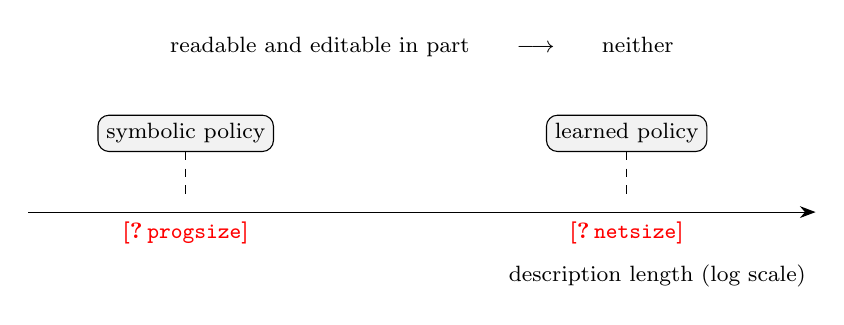
\begin{tikzpicture}[x=1cm,y=1cm]
  \draw[-{Stealth[length=2mm]}] (0,0) -- (10,0);
  \node[anchor=north east,font=\footnotesize] at (10,-0.55)
    {description length (log scale)};
  \node[draw,rounded corners,inner sep=3pt,fill=black!5] (p) at (2,1)
    {\footnotesize symbolic policy};
  \node[draw,rounded corners,inner sep=3pt,fill=black!5] (n) at (7.6,1)
    {\footnotesize learned policy};
  \draw[dashed] (p) -- (2,0.15);   \draw[dashed] (n) -- (7.6,0.15);
  \node[below] at (2,0)   {\footnotesize \val{progsize}};
  \node[below] at (7.6,0) {\footnotesize \val{netsize}};
  \node[align=center,font=\footnotesize] at (5,2.1)
    {readable and editable in part \hspace{4mm} $\longrightarrow$ \hspace{4mm}
     neither};
\end{tikzpicture}
\caption{Where the two paradigms sit on the description-length axis, at
comparable playing strength. \emph{Schematic; both values are placeholders.} The
comparison is not that one paradigm is smaller but that the difference is one of
scale, which is what makes description length the variable this paper measures.
The strength condition is load-bearing: a size comparison between policies of
different strength says nothing.}
\label{fig:size}
\end{figure}

但这种优势需要持续的人力投入。增加规则并不难，难的是不断检查它是否破坏已有行为；程序越复杂，维护所需的人力越多。瓶颈不是程序不能表达，而是维护需要人力，无法长期持续投入。

\begin{center}
\fcolorbox{brandaccent}{white}{\parbox{0.93\linewidth}{\small
\textbf{观察 2：维护需要人力。} 程序的持续修改依赖人力；当人力无法长期投入，策略改进就会停止。}}
\end{center}

多人对抗环境高度变化：对手策略不断切换，使每一种局面都只能获得有限样本。没有对手的单机游戏中，RL 面对近似不变的环境，反复采样相对容易；而在对手多变、样本稀疏的环境中，单纯拟合每种行为模式很难充分学习。此时，从每条轨迹中提取结构并直接优化程序，能够把一次观测中的信息迁移到后续决策，因而更适合少样本条件。

LLM-based coding agent 可以同时利用并弥补前述两点。程序本身是高度启发性且可解释的输入；agent 读取逐决策的轨迹回放来维护程序。轨迹、程序与 policy 修改构成一条信息传递链：若中间表示不能保留决策细节，信道容量就会很低；程序形式则把这条链条直接打开，使回放中的信息能够指向具体规则并落实为局部修改。与此同时，agent 可以持续修改同一个可执行、可读、可局部编辑的程序，逐步承担原本需要人力完成的维护工作。

\begin{center}
\fcolorbox{brandaccent}{white}{\parbox{0.93\linewidth}{\small
\textbf{观察 3：LLM agent 的闭环作用。} 直接读取程序提供高度启发性、可解释的输入；结合轨迹回放，agent 获得宽信息通道来维护程序，并逐步承担原本需要人力的持续维护。}}
\end{center}

% THE NAMING AND THE CONCESSION, moved here from 02-preliminary.tex on 2026-08-20 when that
% section was deleted. The paragraph above already argued the channel is wide; what only
% existed in Section 2 was the NAME and the limit on what the name licenses. Both have to
% survive, and this is the last paragraph that can carry them -- Section 3.3's "observation
% trace" and Section 4's replay contract both use the term as though it were defined.
%
% THE CONCESSION IS THE POINT, and it must not be softened into a hedge. The channel's width
% is a property of what is available and of the agent reading it, NOT of the policy being
% symbolic: echo2025hindsight rewrites failed episodes into a memory, holds no program
% anywhere, and gets the same kind of per-sample gain. So the paper states two bounds over
% two different objects and never merges them -- lower over what the loop can read, where
% the symbolic form earns no credit; upper over what the loop can edit, where the program is
% answerable. Merging them is what produces the unsupportable version of the claim, and a
% reader will supply the merged version unaided if this is left loose. 01-introduction.tex
% already concedes the same limit; keep the two statements consistent if either is edited.
这里的“宽信道”需要轨迹提供丰富的决策信息，也需要程序形式把这些信息完整传递到 policy 修改；没有程序、只把失败经验写入记忆的循环也可能获得部分类似的信息增益~\citep{echo2025hindsight}。本文真正要测量的是：在对抗式游戏的少样本条件下，这条信息链能否通过一个可解释、可持续修改的程序转化为策略性能。

\end{CJK*}

\subsection{Introducing Adversarial Heuristic Learning}
\label{sec:hl-method}

We use \emph{Adversarial Heuristic Learning} (\ahl) for the following setting:
an agent iteratively edits one executable policy, receives decision-level traces
from matches against changing external opponents, and is scored by a referee-side
evaluation pool it cannot rewrite. AHL is therefore the adversarial-game
instantiation studied here, rather than a definition of heuristic learning in
general. The policy artifact persists across rounds; each revision is made from
the current program, the game rules, and the feedback collected so far.

The instantiation is a loop between two agents, and it is deliberately simple. A
\emph{policy agent} is the program under revision; it plays the game and produces
interaction traces. A \emph{generative agent} observes those traces, together with
the rules and the policy agent's own source, and either generates a policy or
revises the one in hand. Its output is the next version of the policy agent, which
is then rescored against the frozen test pool, and the loop repeats.
Algorithm~\ref{alg:loop} states it in full.
The complete overview, including the contest-game suite in which the loop is measured,
is shown in Figure~\ref{fig:hl-arena-overview}.

% REPLACED the tikz block diagram with this algorithm block on 2026-08-19 at the
% user's direction. The diagram drew three boxes and three arrows, which is what the
% prose already says; the algorithm carries what the prose cannot -- the order of
% operations, where the budget is decremented, what is logged, and the fact that the
% generative agent's two modes are one call site with different inputs.
%
% Kept deliberately short, because the user's framing of the loop is "就这么简单".
% Resist adding the description-length protocol, the KL measurement, or the budget
% conversion here; those are separate protocols and belong in their own paragraphs
% later in 3.2. An algorithm that grows past one column stops being the thing that
% makes the loop look simple.
%
% [b] for the same reason as Figure 1: with [t] the float landed above its own
% subsection heading, inside the tail of 3.1. Check the rendered page after any edit
% above it.
\begin{algorithm}[b]
\caption{Heuristic learning. A generative agent observes the interaction between
the policy agent and its environment, then generates or revises the policy agent.
One revision per iteration; every version, score, and trace is appended to the log.}
\label{alg:loop}
\begin{algorithmic}[1]
  \Require game rules $R$, training pool $\mathcal{O}_{\text{train}}$, frozen test
    pool $\mathcal{O}_{\text{test}}$, budget $B$
  \State $\pi_0 \gets \Call{Generate}{R}$
    \Comment{no policy in hand: the agent writes one}
  \State $\mathcal{L} \gets \langle\,\rangle$
    \Comment{append-only log}
  \For{$t = 1$ \textbf{to} $B$}
    \State $\tau_t \gets \Call{Play}{\pi_{t-1}, \mathcal{O}_{\text{train}}}$
      \Comment{interaction traces, including the losses}
    \State $\pi_t \gets \Call{Revise}{\pi_{t-1}, R, \textsc{src}(\pi_{t-1}), \tau_t}$
      \Comment{reads; then edits}
    \State $e_t \gets \Call{Score}{\pi_t, \mathcal{O}_{\text{test}}}$
      \Comment{Elo on the frozen pool}
    \State append $(\pi_t, e_t, \tau_t)$ to $\mathcal{L}$
  \EndFor
  \State \Return $\mathcal{L}$
    \Comment{the trajectory is the result, not $\pi_B$ alone}
\end{algorithmic}
\end{algorithm}

We use one revision per iteration and append every policy version, score, and trace
to the log so that changes remain attributable.

\subsection{Key Elements of AHL}
\label{sec:hl-bottleneck}

Algorithm~\ref{alg:loop} has two elements that determine what AHL can learn. The
maintenance rule determines whether feedback can be written into the persistent
program continuously and effectively. The feedback information determines how much
the agent can observe in each round, including which opponents it plays and which
parts of each interaction are recorded.

\paragraph{Maintenance rule.}
The rule controls how revisions are proposed, checked, accepted, and remembered.
It must prevent a fix for one opponent from silently breaking behaviour that already
works against others, while retaining rejected changes so that the loop does not
rediscover them. Rescoring each revision against a fixed reference and logging the
decision makes the maintenance process attributable; its stability is an empirical
question evaluated in Section~\ref{sec:experiments}.

\paragraph{Feedback information.}
The feedback contract controls the input channel. Outcome-only feedback forces the
agent to guess which rule caused a loss, whereas decision-level traces expose the
sequence of actions, opponent replies, and the turning point needed to edit a
specific rule. In adversarial games, the opponent pool is part of this contract:
the agent can only learn from failures that the selected opponents elicit. Thus both
who the policy plays and what each replay contains determine the information
available for the next revision; our concrete trace is specified in
Section~\ref{sec:benchmark}.

% ---------------------------------------------------------------------------
% Benchmark
%
% RENAMED from "Experiments" on 2026-08-19. This section is now the benchmark
% itself -- the archive, the games, the apparatus, the protocol -- and the
% findings live in 05-experiments.tex. Setup only; no result may be stated here.
%
% NAMED \benchname (HL-Arena) on 2026-08-19; the macro is defined in main.tex with
% the rename rationale. This section is where the name is introduced properly --
% what it contains, not whose method it serves. Write the contents, because the
% name says "HL" and the arena is not HL's: human submissions across \val{editions}
% editions, RL baselines run inside it, classic games as structural controls, three
% opponent pools. If the section reads as though it were built for HL, the name has
% made the comparison look pre-decided, which is the one failure mode it carries.
% Never "our HL benchmark"; never gloss the HL as the thing being measured.
% The heading is \section{\benchname} as of 2026-08-19 at the user's direction --
% the word "Benchmark" is gone from it, so the name has to carry the section on its
% own and the opening sentence must say what \benchname IS before doing anything
% else. The label stays sec:benchmark: it is referenced from 01-introduction.tex
% (the pretraining-objection pointer) and renaming it buys nothing.
% Note the label move that came with the rename: sec:experiments now names the
% RESULTS section, and the introduction's pretraining-objection pointer was
% repointed to sec:benchmark because the contamination check it promises is
% specified and run here.
%
%   - models and scaffolds under test; which are held fixed across games.
%   - the baseline choice and *why*, restated here rather than assumed from the
%     introduction. Comparing HL against policy gradient alone confounds
%     symbolic-vs-neural with on-policy-vs-off-policy: policy gradient uses a
%     batch once and discards it, while HL is off-policy and cross-policy-class
%     (it learns from any opponent's replays and from human source). So
%     model-based RL is the primary baseline and policy gradient is the
%     on-policy reference point, not the headline comparison. A referee who
%     only sees a policy-gradient baseline is right to discount the result.
%     Cite offpolicyvaluellm2026 and samplereuse2022 where the distinction is
%     drawn.
%   - the budget ledger. This table is what answers the selection-effect
%     objection raised in the introduction, so it needs every denominator:
%     environment steps, coding_agent_act calls, tokens, dollars, wall-clock.
%     Report HL and RL in all of them, including the ones where HL loses
%     (\val{loseaxis}).
%   - the frozen evaluation set and the three opponent pools; how Elo anchors
%     stay comparable across games and across editions. Cite asro2026coevolution
%     here: it is the nearest neighbour on pool design (LLM best-response oracles
%     over a growing strategy pool in a two-player zero-sum game), and the
%     contrast worth drawing is that its pool grows by construction while ours is
%     frozen at test time -- we buy comparable Elo within a run and give up
%     co-evolutionary pressure, which is a design choice to defend rather than
%     omit.
%   - RL budget ceiling: to claim a crossover at \val{crossover} the baselines
%     have to actually be run past it. If they are not, report a lower bound
%     ("no crossover within X steps"), never an extrapolation.
%   - the transfer suite: \val{ntransfer} further benchmarks, no retuning.
%   - seeds, repeats, and how variance is reported.
%   - a contamination check, which the introduction currently PROMISES twice and
%     no section yet delivers. The intro claims the archive is contamination-
%     resistant because the venue predates the benchmark, and leans on the same
%     property to answer the pretraining objection ("pretraining supplies general
%     programming competence rather than knowledge of these games"). That is an
%     empirical claim about a specific model's training data and cannot be
%     asserted from the venue's history alone -- the archive is a public web
%     artifact, so its games and possibly its submissions may well be in a
%     pretraining corpus.
%     olympiad2025percentile has the protocol worth copying: temporal splits
%     (pre- vs post-cutoff editions), familiarity probes (ask the model to state
%     the rules unprompted), perturbation (change a rule and check the policy
%     degrades as a fresh solver would rather than as a recalled one), and
%     code-similarity against archived submissions. Copy their closing caveat
%     too: these make direct copying unlikely and do not rule out exposure to
%     related material. If a familiarity probe shows the model already knows a
%     game, that game is reported separately, not dropped.
%
% THE PROVENANCE ARGUMENT LANDED HERE on 2026-08-19, moved out of
% 02-preliminary.tex when that section was written. It had been parked in 02 since
% 2026-08-18, which predates 04 becoming \benchname and taking ownership of the
% archive; provenance argues why this venue is worth building a benchmark on, so it
% belongs in the section that presents the benchmark. 02 kept only the VOCABULARY
% (percentile, human state of the art, the three pools, distribution vs reference)
% and defines each without arguing from it. Two halves to write here, and note that
% the second half of the first one is already covered above by the contamination
% check -- what is missing is the positive argument, not the caveat:
%   - Contamination resistance, as a property this venue has for free. The contrast
%     is livecodebench2024 and workbuddybench2026, which buy it by authoring fresh
%     tasks or collecting them continuously -- a cost paid forever, every time the
%     benchmark is refreshed. Here it falls out of a venue that predates the
%     benchmark and was never built for evaluation. State the limit in the same
%     breath: the archive is PUBLIC, so provenance is not proof, which is why the
%     check above exists. Never write that the rules are absent from pretraining
%     data; that inference was removed from 01-introduction.tex and from
%     06-discussion.tex already, and 02 was told not to reintroduce it.
%   - A distribution rather than a reference solution. Thousands of independent
%     attempts at the same games is what licenses percentile placement at all;
%     mlebench2024 (Kaggle) and olympiad2025percentile are the precedents for
%     reporting a method as a percentile of a real human field. This is what the
%     human baseline in contribution 3 rests on.
% All three of livecodebench2024, workbuddybench2026, and mlebench2024 are ORPHANED
% as of 2026-08-19 -- registered in refs.bib, cited nowhere in body text -- and this
% is the only place they have a home. If this paragraph is cut, cut the keys too.
%
% ===========================================================================
% THE PLATFORM'S OWN SOURCE WAS READ ON 2026-08-19, and it contradicts four numbers
% this paper already asserts. Cloned to _platform/ (gitignored; see .gitignore for
% why it is not a submodule): git@github.com:Aoraku/AgentBench.git, 19 commits, last
% 2026-08-17. NOT the AgentBench of arXiv 2308.03688 -- same name, unrelated project,
% and Section 4 must say which one it is wherever it names the platform.
%
% Counts below are off the nine per-game players/manifest.tsv files. One parsing note
% that cost a wrong number once already: the manifests are CRLF, so awk on the last
% field compares against "true\r" and silently returns zero. Strip \r before counting.
%
% WHAT THE ARCHIVE ACTUALLY CONTAINS, per game (versions / unique users / rank
% anchors), summed to 5004 submission versions:
%   generals 752/31, snakego 678/17, antwar 644/21, antwar2 631/21, deepclue 625/22,
%   miracle 569/17, aquawar 534/12, rollman 309/20, lostspace 251/17.
%   RECOUNTED 2026-08-19, same day: the totals above and the "9 rows with an empty
%   split" below were BOTH wrong, from one cause. The manifests carry a header line
%   plus a block of "#" comment lines documenting the columns, and `tail -n +2` skips
%   only the header, so comment lines were counted as submission rows. Correct counts,
%   filtering '^#' / header / blanks:
%     generals 752/30, snakego 678/16, antwar 644/20, antwar2 631/20, deepclue 625/21,
%     miracle 569/16, aquawar 534/11, rollman 309/19, lostspace 251/16
%     = 4993 registered rows (not 5004), from 143 unique usernames GLOBALLY
%     (the per-game user counts sum to 169, so ~26 people entered more than one game).
%   The split covers the archive exactly: 778 train / 4215 test = 4993. There are NO
%   unsplit rows; that finding was an artifact of the same miscount and is withdrawn.
%   One real gap remains: 52 registered rows have NO directory on disk (all of them
%   anonymous entries), so the playable pool is 4941, not 4993. Registered scale and
%   playable pool are different numbers and the section must not use one for the other.
%
% FOUR CONFLICTS, in ascending order of how much they cost:
%   1. \val{nsub} says ~10,000. The archive holds 5004 submission versions. Roughly
%      2x too high. Fix the key, and decide what the unit is: 5004 counts VERSIONS,
%      each kept as an independent testcase, which is the platform's own convention.
%      "Submissions" in the paper's sense may well mean versions, but say so.
%   2. \val{nmatch} says ~100,000 matches. THERE IS NO MATCH ARCHIVE IN THIS REPO.
%      The 712 replay-ish files under players/pool/ are contestants' own local test
%      leftovers (mini_replay.txt inside submission directories), not recorded contest
%      games. Matches are something the evaluator RUNS, not something the archive
%      supplies. So nmatch is either a number we generate ourselves (in which case it
%      is an experimental cost, belongs in the budget ledger, and must not be quoted
%      as archive scale) or it must be dropped. As written the abstract credits the
%      archive with it.
%   3. \val{editions} says the archive spans 30 editions. Each game belongs to exactly
%      ONE edition, and the nine span editions 24-30 -- SEVEN editions. 30 is the
%      latest edition number, not the span, and the venue being 30 editions old
%      (founded \val{founded}) is a fact about the venue, not about our archive. The
%      abstract's "archive ... spanning \val{editions} editions since \val{founded}"
%      is wrong on the archive as we hold it. Either add a key for the archive's span
%      (7) and keep editions for the venue's age, or restrict the claim.
%      This also kills the folk-ordering test as 02-preliminary.tex states it: "Section
%      5 reports what 30 editions of outcomes say" cannot be run across 30 editions
%      when we hold 7, and with one game per edition, paradigm composition over
%      editions is confounded with the game changing underneath it.
%   4. THE PERCENTILE CLAIM IS THE EXPENSIVE ONE. The pools are FINALS LADDERS
%      (决赛天梯 / top_algorithms/corpus/<ed>_<game>_final*), not all entrants. Per
%      game there are 12-31 unique users. Of 5004 versions, 183 carry a rank anchor
%      and 153 carry an Elo; 3501 are fully anonymous, 1320 named but unranked. So
%      "thousands of independent attempts at the same games", which is what
%      licenses percentile placement in the provenance argument above, is not what
%      this is: it is ~20 finalists per game, each with many versions. \val{pct} as
%      "the XXth percentile of the field" therefore means percentile of a FINALS
%      field, which is a much stronger opponent set and a much smaller one. That is
%      arguably a better result and definitely a different claim; it must be stated as
%      the finals field everywhere, and mlebench2024/olympiad2025percentile are
%      precedents for percentile-of-a-full-field, so leaning on them needs care.
%      Versions-as-testcases also means the field is not independent: 5004 versions
%      from ~200 user-game pairs are heavily correlated, so any percentile or Elo
%      computed over versions must say what the unit of independence is.
%   5. THE SUITE CONTRADICTS 02-preliminary.tex's OPENING DEFINITION, which is the
%      most structural conflict of the six. That paragraph reads "a game is a
%      two-player adversarial game of perfect information". Of the nine:
%      lostspace is FOUR-player and the platform's own edition table calls it
%      多人非零和 (multiplayer NON-zero-sum); aquawar is built on 隐匿信息 and
%      identity assertion, i.e. IMPERFECT information; lostspace is additionally
%      局部可观测 (partially observable); deepclue is a SINGLE-player scripted
%      reasoning task driven through an LLM API; rollman is role-ASYMMETRIC
%      (rollman vs ghost). So the definition covers roughly four of nine games.
%      "zero-sum", "perfect information" and "two-player" each appear exactly once
%      in the body, all in that one sentence, so this is cheap to fix and must be:
%      either narrow the suite actually analysed and say which games are excluded
%      and why, or widen the definition and drop the perfect-information
%      assumption. Do NOT leave it as is -- a reader who checks the game list will
%      find the paper's central definition false of most of its own benchmark.
%      Note this also touches Section 3.3's trace argument, which says the trace can
%      only exhibit failures an opponent elicits: under imperfect information the
%      trace additionally cannot show what the opponent knew, which is a sharper
%      version of the same bottleneck and worth one clause there once the scope of
%      the suite is settled.
%   6. THE EDITION QUESTION IS SETTLED by docs/清华计算机系智能体大赛历届资料表.md,
%      which is the platform's own edition-level index and should be cited as the
%      source for any venue-scale claim. It states the venue was founded 1997 with
%      2023 as the 27th edition, so \val{editions}=30 and \val{founded}=1997 are
%      both right ABOUT THE VENUE. But it also records that editions 1-22 have
%      insufficient publicly verifiable material (years inferred from the founding
%      date alone; no rules, code, standings, or replays) and that edition 23 (2019,
%      DOTO) survives only as public GitHub repos and is NOT among our nine games.
%      Verifiable assets therefore begin at edition 24. That is the number the
%      archive sentence needs, and the table is the citation for it.
%   Also: Elo is sparse and NOT on one scale. deepclue's max "elo" is 28859 and
%   rollman's are all 0, so the column is whatever each ladder recorded. Elo anchors
%   have to be recomputed by our own evaluator before any cross-game Elo is quoted;
%   \val{elogap} and the human-SOTA comparison both depend on this.
%
% WHAT THE PLATFORM GIVES SECTION 4 FOR FREE, and it is a lot:
%   - Nine games, each with rules.md, decision_space.yaml, replay_format.md, a
%     runnable evaluator/, plugin.py, and players/pool/ + manifest.tsv. Games:
%     antwar2(30), deepclue(30), rollman(29), generals(28), antwar(27), snakego(26),
%     lostspace(25), aquawar(25), miracle(24). \val{ngames}=9 CHECKS OUT.
%   - Player counts per match vary (lostspace is 4-player, deepclue single-player
%     scripted, rest 2-player), and generals has two tracks (popular/advanced).
%     "Two-player zero-sum" as a blanket description of the suite is false; either
%     scope the claim or report the exceptions.
%   - deepclue depends on an external LLM API and returns infra_error without it.
%     A game whose evaluator needs an LLM to run is a confound for a paper comparing
%     an LLM-driven method against RL. Report it separately or justify keeping it.
%   - THE TRACE CONTENTS 3.3 SAYS ARE A DESIGN VARIABLE ARE SPECIFIED HERE:
%     docs/replay-format-spec.md plus each game's replay_format.md. 3.3 promises
%     Section 4 states what our tau_t contains, so write it from these.
%   - docs/evaluator-contract.md and docs/metrics-schema.md are the apparatus
%     contracts; the three-repo split (A assets / B HL / C RL) means the RL baseline
%     runs inside the same arena, which is what makes the budget ledger comparable.
%   - Rules are derived from the official backends in backend_sources/, so rules.md
%     is a restatement, not the authority. If the paper quotes a rule, cite the
%     backend as the source of truth.
% ===========================================================================
%
% 01-introduction.tex's "a distribution of human skill to place a method within"
% still forward-references sec:preliminary, deliberately: that sentence is about
% what the archive supplies, and the term is defined there. If the paragraph written
% here ends up carrying that sentence's weight instead, repoint it.
% ---------------------------------------------------------------------------

% ===========================================================================
% WRITTEN 2026-08-19 at the user's direction: "现在你先大概介绍HL-Arena是啥东西就行,
% 比如里面的来源, 比赛的格式, 统计的数据, 评测的逻辑" -- provenance, contest format,
% archive statistics, evaluation logic. Four subsections in that order. Deliberately
% NOT written yet, because they are apparatus for OUR runs rather than description of
% what the arena is, and no run exists: the budget ledger, the transfer suite, seeds
% and variance, the contamination check, the model/scaffold table, and the baseline
% rationale. All six are still owed and their scope notes above stand.
%
% EVERY NUMBER HERE IS MEASURED off the platform repo, not from the proposal. Three
% claims the paper made before this section was written are contradicted and are NOT
% repeated: \val{nsub} (~10,000, about 2x high), \val{nmatch} (~100,000 matches, which
% the archive does not contain at all), and \val{editions} as the archive's span.
% \val{nmatch} is not cited anywhere in this section on purpose -- matches are what the
% evaluator runs, so that number is an experimental cost for the budget ledger.
%
% THE TABLE IS THE SOURCE OF TRUTH for per-game counts and they are literals there
% rather than \val keys, which is a deliberate exception to the numbers.tex rule: nine
% games x six columns would be 54 keys used once each. Anything quoted in PROSE, here
% or elsewhere, must be a key. If a per-game number is ever needed in a sentence,
% promote that one to a key rather than inlining it.
%
% THE SUITE'S HETEROGENEITY IS STATED OUTRIGHT in the second paragraph of the games
% subsection, because 02-preliminary.tex still opens "a game is a two-player
% adversarial game of perfect information" and that is false of five of the nine. This
% section does not paper over it: the information column shows it and the prose names
% the exceptions. 02 still has to be narrowed -- that is conflict 5 above and it is not
% fixed by this section, only made impossible to miss.
%
% ANONYMITY: the venue is described by properties only, never named, and the edition
% table is cited as a platform document with no URL. The game names are kept, and they
% are the residual de-anonymisation risk recorded in main.tex -- they are recoverable
% to the venue by search. Keeping them is a judgement call: without them the suite
% cannot be described concretely enough for a reader to judge the benchmark. If the
% risk is ruled unacceptable, the fix is to letter the games (G1--G9) and keep the
% property columns, NOT to delete the table.
%
% NO RESULT IS STATED HERE, per the split with 05-experiments.tex.
% ===========================================================================

\section{\benchname}
\label{sec:benchmark}

\begin{CJK*}{UTF8}{gbsn}

\subsection{规则描述}
\label{sec:arena-formulation}

一个 arena 实例表示为 $(G,R,A,F,H)$：其中 $G$ 是游戏，$R$ 是固定规则，
$A$ 是与角色相关的动作空间，$F$ 是判别器（referee），$H$ 是存档中的人类选手集合。
策略读取其角色可见的状态并返回一个合法动作；判别器执行对局并返回结果与回放。
AHL 在每轮接收 $(R,A)$、当前程序和训练回放，并输出修改后的程序；程序是跨轮次
持续保留的对象。

\benchname 是一个由存档支持的竞技场，包含 \val{ngames} 个竞争性游戏；每个游戏都提供
固定规则、机器可读的动作空间、可运行的判别器以及人类编写的程序（共 \val{nsubv} 个版本）。
这些游戏和排行榜早于本文研究；我们只为存档程序和本文方法增加统一的评测器。

% THE SCOPE DEFINITION NOW LIVES HERE, moved from 02-preliminary.tex on 2026-08-20 when
% that section was deleted at the user's direction ("Preliminary删了吧，目前看起来没有定义
% 啥好的符号"). It is one of the four places that carry this paper's scope limit -- the
% title, one sentence in the abstract, two in Section 1, and this paragraph -- and the
% comment at the head of main.tex names all four. If this paragraph moves again, update
% that comment in the same edit or the count silently goes wrong.
%
% WHAT THIS DEFINITION REPLACED, kept because the error is easy to reintroduce: the old
% text read "a game is a two-player adversarial game of perfect information", which is
% FALSE of five of the nine games below -- LostSpace is four-player and not zero-sum,
% AquaWar hides each side's roster, LostSpace and Rollman are partially observable,
% Rollman's two roles are asymmetric and separately ranked, DeepClue is single-player.
% The heterogeneity paragraph in 4.1 is the detailed statement; this is the definition
% written so as not to contradict it.
%
% KEEP IT THIS SHORT. A four-numbered-condition version with a page of argument about
% what each condition supplies the loop was written on 2026-08-19 and cut the same day
% ("就说我们在博弈类上面打，就行"). The three requirements below are the ones a claim in
% this paper actually rests on, and the sentence after them earns its place because
% dropping two-player / zero-sum / perfect-information is exactly what makes the
% definition true of our suite rather than true of chess.
%
% The legality clause is here rather than in the definition because it is the one part
% auditable in the arena's own files rather than asserted: every game ships a legal-move
% specification with the predicate that decides it (legal_actions plus
% policy_interface.legality in all nine decision_space.yaml files), and every game is
% adjudicated by the evaluate() contract.
在本文中，\emph{game} 具有固定规则；\emph{policy} 读取其角色可见的
状态并返回合法动作；外部判别器则在其无法控制的对手集上进行评分。这组游戏包含多人、
非零和、部分可观测和角色不对称的情况，因此本文不作更强的游戏假设。每个游戏都提供
合法性规范和判别器协议，保证对局双方均可审计。

\subsection{比赛内容与来源}
\label{sec:arena-provenance}

这些游戏来自一个年度计算机智能体竞赛。每届比赛发布一个游戏的规则与运行套件，
进行持续数月的排行榜对局，并保留选手反复提交的每个版本。因此，存档记录的是
真实人力预算下的程序维护轨迹，而不只是最终方案。

公开且完整的资源从第~\val{edfirst}~届开始，因此 \benchname 覆盖
\val{edfirst}--\val{edlast}：共七届、\val{ngames} 个游戏。该竞赛早于本文基准，
并非为模型评测而设计，因此可以提供有用的污染检查，但不能证明数据完全独立
\citep{livecodebench2024,workbuddybench2026}。

表~\ref{tab:games} 总结了这组异质游戏，涵盖网格与领地争夺、生存、隐藏身份以及
脚本化问答等任务。每个游戏的具体规则、动作空间和回放格式见附录~\ref{app:arena}；
附录~\ref{app:case} 进一步完整展示其中一个游戏的实例。

% [b], not [t], for the same reason as Section 3's two floats: with [t] this table
% lands at the top of the page and sits ABOVE the \subsection{The games} heading that
% introduces it, so the reader meets the suite before being told what they are looking
% at. Verified on the rendered page -- grep cannot catch this. Do not "tidy" it to [t].
\begin{table}[b]
\centering
\small
\begin{tabular}{llccrr}
\toprule
Game & Ed. & Players & Information & Versions & Entrants \\
\midrule
Miracle    & 24 & 2 & perfect   & 569 & 16 \\
AquaWar    & 25 & 2 & imperfect & 534 & 11 \\
LostSpace  & 25 & 4 & partial   & 251 & 16 \\
SnakeGo    & 26 & 2 & perfect   & 678 & 16 \\
AntWar     & 27 & 2 & perfect   & 644 & 20 \\
Generals   & 28 & 2 & perfect   & 752 & 30 \\
Rollman    & 29 & 2 & partial   & 309 & 19 \\
DeepClue   & 30 & 1 & partial   & 625 & 21 \\
AntWar2    & 30 & 2 & perfect   & 631 & 20 \\
\midrule
\multicolumn{4}{l}{Total} & \val{nsubv} & \\
\bottomrule
\end{tabular}
\caption{\benchname 中的 \val{ngames} 个游戏及其竞赛届次。Versions 统计存档的提交版本数；
Entrants 统计该游戏中产生这些版本的不同实名选手数，但不求总和：存档中多数记录匿名，
无法跨游戏关联身份，因此该字段只能作为规模上界。具体统计见附录~\ref{app:arena}。}
\label{tab:games}
\end{table}

% The suite's spread across these properties is why Section 2's definition does not
% require two players, zero sum, perfect information, or symmetric roles -- it would be
% false of five of these nine games. DeepClue is the one that falls outside the definition
% itself (single-player, and requires_llm_api: true so its referee calls a language
% model), which is why it is reported apart; that is a consequence of the definition, not
% an exception to it. Do not let a later edit quietly fold DeepClue into the main claim.
这组游戏的差异既拓宽了结论的适用范围，也限制了可以作出的统一表述。LostSpace 是四人
且非零和；AquaWar 隐藏双方身份信息；LostSpace 和 Rollman 部分可观测，因此回放记录的
是角色当时能看到的内容，而不是完整局面；Rollman 的两个角色不对称并分别排名。DeepClue
是单人脚本化推理任务，其判别器还会调用外部语言模型，因此没有对手和固定判定机制；这对
比较语言模型方法与强化学习也构成混淆，我们单独报告它而不删除它。凡是需要二人零和假设
的结论，我们会明确列出适用的游戏。

% STRUCTURAL CONTROLS, moved here from 02-preliminary.tex on 2026-08-20 with the rest of
% that section. It has to survive somewhere: 01-introduction.tex's contribution 2 promises
% "classic games as structural controls" as part of the apparatus, and this is now the only
% place the paper says what they control FOR. Without that sentence the word "control" is
% decoration -- which is why it is spelled out rather than named.
% These games are NOT in Table 1 and must not be added to it: the table is the contest
% suite, \val{ngames} counts the contest's own games, and folding the classics in would
% break every per-game count in this section.
除竞赛自身的游戏外，我们还保留国际象棋、围棋等具有独立研究传统的经典游戏作为结构
控制。它们用于检验复杂度测量是否只对本套游戏成立：这些游戏的策略复杂度已有外部依据，
因此可以校准第~\ref{sec:hl-motivation} 节中的复杂度代理指标，并为跨游戏排序提供参照。

\subsection{存档与参赛程序}
\label{sec:arena-archive}

每个提交都是一个带版本号的源代码快照，并对应 manifest 中的一行记录。我们统计的是版本，
而不是人数：身份信息不完整且版本之间存在相关性，因此百分位数必须注明独立性单位。
只有可运行的快照进入对手池，并保留存档中的开发集/留出集划分。

版本索引为人类维护过程提供统一的修订次数；其分布和注意事项见附录~\ref{app:human}。

排行榜中的选手是决赛子集，存档中的原始分数仅用于溯源；本文会根据统一协议重新计算
所有分数和程序规模指标。

% THE AUDIT CRITERION AND THE FOLK ORDERING, moved here from 02-preliminary.tex on
% 2026-08-20. Both belong to this subsection rather than to a vocabulary section: they are
% how the archive gets classified, and the classification is a result this paper reports.
%
% WHY THE CRITERION MUST BE DECIDABLE, and why it is worth the sentences it costs:
% \val{pheur} and \val{prl} appear in the abstract and in Section 1, and they are worth
% exactly as much as this definition is. Classifying the winners is also how RQ3 gets
% answered, so it is not bookkeeping.
% The hand-tuning clause is the load-bearing half. Without it the category swallows every
% serious entry and measures nothing, because a contestant who tuned coefficients over a
% season of ladder matches has run an optimization loop -- with themselves as the
% optimizer. That is the distinction the clause draws, and it is a distinction about WHO
% the optimizer is, not about how much evidence informed the tuning.
%
% THE FOLK ORDERING WAS FIRST DRAFTED IN THE PROHIBITED REGISTER and fixed the same day.
% It read "Practitioners in this venue have long ordered approaches by expected ceiling",
% which is the received-opinion framing the user prohibited twice ("不要说什么'一般别人觉得
% 怎么样'，这样写论文不够严谨"). Treat that ban as global -- it was given for
% 01-introduction.tex and has now resurfaced in three other files. Two things make the
% present version defensible: it attributes the ordering to nobody, and it is stated as a
% hypothesis with a consequence the archive can check. There is also a factual reason the
% old wording could not stand: nothing in this repo establishes what this venue's
% contestants believe, so "have long ordered" asserted an unmeasured fact about a
% population. Section 1 states the ordering itself; what is added here is the consequence,
% which is what makes it testable rather than a piece of framing.
只有当拟合参数或拟合过程实际影响动作选择时，我们才将提交归类为 learned；手工调节的
系数仍归为 heuristic。这样，类别统计可以被复核，而不依赖于提交者如何命名自己的方法。
% FIXED ON THE WAY IN, 2026-08-20. The sentence in 02-preliminary.tex read "reports what
% \val{editions} editions of outcomes say", and \val{editions}=30 is the VENUE's age, not
% this archive's span -- numbers.tex carries the standing instruction "Never use editions to
% describe the archive again -- that was the error". The audit runs over what we hold, which
% is editions \val{edfirst}--\val{edlast}, seven of them. Two other body uses of the same key
% are still wrong for the same reason and are NOT fixed here because they are the unresolved
% archive-scale conflict awaiting the user's decision: 01-introduction.tex's "finals in
% \val{nrlfinal} of \val{editions} editions" and the abstract's "spanning \val{editions}
% editions". Fix all three together when that decision lands.

\subsection{双方对局的评测协议}
\label{sec:arena-eval}

所有游戏都通过统一的判别器接口评测：带有随机种子的请求固定参赛程序与角色，
判别器执行对局并返回分数、胜者和回放。代码在沙箱中运行；对于非对称角色，交换双方
角色并成对评测。

对局成功与否由判别器的最终结果决定：非法动作、超时或程序崩溃均判为该方失败；
基础设施故障则重新运行，不计入选手结果。

回放记录每个角色在每一步可见的状态、合法动作集合、实际选择的动作及其是否被接受，
并不泄露隐藏状态；这正是 AHL 使用的训练轨迹，具体格式见附录~\ref{app:case}。

\subsection{排行榜分数}

对于每一场对局，胜者得分 $S=1$，败者得分 $S=0$；若判别器返回平局，双方均得
$S=1/2$。给定当前评分 $r_i,r_j$，选手 $i$ 的预期得分为
\[
E_i=\frac{1}{1+10^{(r_j-r_i)/400}},
\qquad r_i' = r_i + K(S_i-E_i),
\]
其中 $K$ 是预先固定的更新系数。排行榜分数是选手在规定对手集上完成全部对局后的
最终 Elo；训练过程中的 AHL agent 不读取该排行榜分数，Elo 只作为训练结束后的评测指标。

% RATINGS, POOLS, AND THE TWO HUMAN QUANTITIES, moved here from 02-preliminary.tex on
% 2026-08-20. This is the paragraph Section 5 depends on most: every number it quotes is
% either an Elo, a percentile, or a comparison against the human state of the art, and
% none of the three means anything without the pool it was computed on. It goes in the
% Protocol subsection because all of it is protocol.
%
% NO ELO CITATION EXISTS. refs.bib still has no elo1978rating or equivalent as of
% 2026-08-20, so the protocol is defined here without attributing the system -- an
% unattributed Elo is the kind of thing a referee notices. Add the key before submission;
% this paragraph is written so the citation drops in after "Elo ratings" without rewording.
%
% THE THREE POOLS ARE ALSO IN Algorithm 1 (\mathcal{O}_train, \mathcal{O}_test as
% \Require) and in Section 7's "frozen test pool drawn from a whole human field". Those
% two uses now depend on this definition. The frozen pool is what makes our Elo comparable
% within a run; the ARCHIVE's human population drifts across editions, which is what the
% anchor pool absorbs. Never write "drifting opponent pool" of the frozen test pool --
% 07-related-work.tex's header carries the same warning for the same reason.
%
% PERCENTILE AND HUMAN SOTA ANSWER DIFFERENT QUESTIONS and the paper reports both. The
% distinction is load-bearing twice over: 01-introduction.tex claims both \val{pct} (a
% distribution) and \val{nbeat} of \val{ngames} (a maximum), and 4.2 above has already
% conceded that our ranked pools are FINALIST fields, so a percentile here is a percentile
% of finalists. That concession and this definition must be read together; do not restate
% the percentile as a percentile of all entrants.
% "Across all editions rather than within one" is the only honest reading of "human state
% of the art" -- it is a bar that rises with every edition, and taking it within one
% edition would let a weak edition supply a cheap win.
排行榜报告的是该判别器计算的 Elo，而不是原始回报。训练集、冻结测试集和人类锚定集
彼此独立；测试集在运行前固定。百分位数衡量方法在存档选手中的位置，人类 state of the art
则取其中最强提交；二者回答不同问题，因此分别报告。

所有实验运行共享同一记录格式：候选程序、参考程序、决策级变化，以及学习、评测和总预算。
同时记录跨方法通用单位和各方法的原生单位；缺失值保持缺失（见附录~\ref{app:apparatus}）。

\end{CJK*}
% CONFLICT RESOLVED HERE, not papered over. 02-preliminary.tex said each ledger is reported
% "in whichever units apply to the method -- environment steps, agent invocations, tokens,
% wall-clock time, currency"; this schema paragraph said "each in tokens and wall-clock".
% Those disagree, and the schema is the one that describes what the apparatus records, so it
% wins on the common units. But the wider list cannot simply be dropped: 01-introduction.tex
% claims a crossover at \val{crossover} ENVIRONMENT STEPS, which is not expressible in
% tokens, and no single unit is native to both an RL learner and an agent maintaining source
% code. Hence the sentence below: common units for every method, plus the native unit where
% one exists. If the apparatus turns out not to record native units, this sentence is the
% thing to fix -- do not fix it by deleting the \val{crossover} claim.
% "The total is the only one comparable across paradigms without qualification" is the
% reason all three are carried rather than just the total: quoting one paradigm's favourable
% denominator is the easiest way to make a budget comparison say nothing.

% ---------------------------------------------------------------------------
% Experiments
% ---------------------------------------------------------------------------
\section{Experiments}
\label{sec:experiments}

We organize the evaluation into five experiments. The first two measure how far AHL
can improve against the human field; the third compares it with reinforcement learning
on a standard game benchmark; the final two isolate the role of opponent selection and
history. Unless stated otherwise, all runs use the same referee, frozen evaluation
pool, and append-only event schema described in Section~\ref{sec:arena-eval}.

\subsection{Fixed-budget performance against human programs}
\label{sec:exp-human}

Under a common revision budget, we run several coding-agent models on every game in
\benchname. For each model and game, we report the initial (raw) Elo, the Elo after
the fixed number of AHL iterations, and the gain. We also place the final policy in
the archived human leaderboard and report its rank and percentile. This experiment
measures cross-model performance at a matched budget rather than the benefit of a
single particularly long run.

\subsection{Long-horizon heuristic evolution}
\label{sec:exp-long}

We select one representative model and run it for a substantially longer horizon,
recording Elo after every revision on a diverse subset of games. The resulting curves
show the initial policy quality, the gains from continued maintenance, the point at
which AHL reaches the human reference, and whether improvement eventually plateaus.
We additionally relate the plateau to the maintained program's description length.

\subsection{AHL versus RL on Go or Chess}
\label{sec:exp-rl}

We compare AHL with established RL baselines on either Go or Chess, using the same
referee-facing interface and matched interaction budgets. The primary plot uses the
number of observed trajectories as the horizontal axis and Elo as the vertical axis;
we report both the final matched-budget Elo and the number of trajectories required to
reach a fixed Elo level. This isolates the sample-efficiency regime in which the
decision-level feedback of an editable program may compensate for the scaling
advantage of a learned policy.

\subsection{Ablation: opponent selection and pool size}
\label{sec:exp-opponent-ablation}

Keeping the model, game, initial policy, and total budget fixed, we vary how AHL
selects the policies that participate in each round and how many policies it samples.
We compare random sampling, agent-selected opponents, easy-to-hard scheduling, and
rank-based selection, together with multiple opponent-set sizes. We report final Elo,
Elo gain, and regression rate to determine whether improvements come from the identity
of the opponents, the diversity of the pool, or simply more matches per round.

\subsection{Ablation: the role of history}
\label{sec:exp-history-ablation}

We compare the standard history-aware agent with a history-free variant. The former
can inspect prior policies, replays, revisions, and outcomes; the latter receives only
the current policy and the latest feedback. All other components and budgets remain
fixed. The difference in final Elo and revision efficiency measures whether sustained
cross-round context is necessary for maintaining a policy rather than merely producing
independent edits.

% ---------------------------------------------------------------------------
% Discussion
%
%   - where each paradigm wins (work item 4). H1-H6: HL at low-to-mid budget
%     when rules are complex and replays interpretable; RL asymptotically when
%     rules are simple, the state space vast, and simulation cheap.
%   - the information-channel asymmetry, stated as a finding rather than as a
%     caveat: rules and replays are a wider channel than a scalar reward, and
%     that is what the budget-conditional result is evidence for. State the
%     scope with it, in the same breath rather than in a later caveat: the
%     channel is what earns the efficiency, so the finding is not that symbolic
%     policies are informationally privileged. A memory-based agent with no
%     program gets a comparable gain (echo2025hindsight). What the program buys
%     is the other bound. Written the loose way, this bullet becomes the
%     paper's most quotable overclaim and the abstract no longer supports it.
%   - the two bounds as one claim, which is the paper's thesis and should be
%     stated here in one paragraph: HL succeeds while K(pi_good) stays under the
%     agent's maintenance capacity. Both the win and the plateau follow from that
%     one inequality, and the reader should leave with it rather than with two
%     separate findings.
%   - the consequence worth drawing out: the ceiling is a property of the
%     maintainer, not of the paradigm, so it moves with model capability. State
%     what that does and does not license. It does not license extrapolating to
%     future models -- we measured one agent generation. It does mean the
%     asymptotic argument against symbolic methods was never about symbolic
%     methods. Resist the stronger version of this; it is the most tempting
%     overclaim available and the easiest to attack.
%   - why language-scale tasks fall outside, in one sentence, from the same
%     inequality: not because they are unstructured, but because no policy of a
%     maintainable description length is any good at them.
%   - what the winning human programs actually contain, and what that says about
%     representation (RQ3).
%   - Limitations, as its own labelled subsection. Two objections are raised in
%     the introduction and have to be answered in full here, not merely repeated.
%
%     Pretraining. The efficiency comparison is between an agent carrying a
%     pretraining corpus and RL starting cold, and no denominator makes that
%     symmetric. What is defensible: environment steps are the scarce resource
%     in a new domain, and the games are the venue's own, so what pretraining
%     plausibly supplies is general coding competence rather than strategy for
%     these games. Word it as plausibility plus a pointer to the Section 4
%     contamination results -- NOT as a consequence of the rules being original,
%     which does not follow (the archive is public) and which the introduction
%     and Section 2 both stopped asserting. This bullet was the last place the
%     provenance version survived; if the check comes back showing familiarity
%     with a game, the honest form here is the conditional one, reporting that
%     game separately rather than resting the limitation on an assumption the
%     data contradicts.
%     Report the figures as conditional on a general-purpose model existing.
%     Do not attempt to amortize pretraining into a per-task number -- any such
%     figure is arbitrary and a referee will say so. If a pretraining-inclusive
%     comparison is wanted, the honest form is a sensitivity statement: how large
%     would the amortized cost have to be to erase the gap?
%
%     The selection effect: the archive's RL scarcity is confounded with student cost
%     structure -- no GPUs, no time, no RL expertise -- so it is evidence about
%     what wins under contest constraints, not about what RL can reach. Say this
%     plainly and cite the budget ledger. Burying it here unlabelled reads as
%     evasion; a reviewer who has to find it themselves will not be generous.
%     Also: single archive, single institution, agent scaffolding held fixed, and
%     Elo anchored across editions whose *human* population changes composition
%     year to year -- a real limitation, and a different pool from HL's frozen
%     test pool, which does not drift. Keep the two distinct wherever both appear.
%   - negative results are in scope and belong here.
% ---------------------------------------------------------------------------

% PRACTICAL GUIDELINES ARE NOW PROMISED HERE, by contribution 3 of the
% introduction as of 2026-08-18 ("From that we derive practical guidelines for
% applying HL -- when to expect it to pay, and when a learned method is the better
% spend"), which forward-references this section. Nothing in the paper delivers
% them yet, and a contribution the paper does not keep is worse than one it never
% claimed. What the guidelines have to be derived FROM, so they are results rather
% than opinions:
%   - the K(pi_good) inequality: expect HL to pay while the winning policy's
%     description length sits below the agent's maintenance capacity. Since
%     \val{maintcap} is measured and roughly game-independent, that is an
%     up-front test a practitioner can apply to a new game by compressing a
%     reference implementation (\val{kproxy}) -- state it that way, as a check
%     someone can run, not as a restatement of the inequality.
%   - the crossover: below \val{crossover} environment steps HL is the better
%     spend, above it model-based RL is. Attach the denominators, because HL costs
%     more \val{loseaxis} and a guideline that hides that is advertising.
%   - the plateau: near \val{plateau} revisions the loop stops paying, so budget
%     for that rather than for indefinite improvement.
% Each guideline must name the result it comes from. If a number is unmeasured the
% guideline does not get stated -- see the numbers guard in AGENTS.md.

% SCOPE SUBSECTION, added 2026-08-19 at the user's direction ("我们在衡量的时候……你要
% 强调并加上一个限定，说明是在这种博弈的情况下"). Section 1 and Section 2 both forward-
% reference this text for what fails outside the class, so it is owed here.
%
% IT CONTAINS NO RESULT OF OURS, deliberately -- it is an argument about the four
% conditions in Section 2 and what depends on each, all of which is established before
% any run. That keeps it writable now, under the numbers guard. Do NOT add a measured
% claim here later; if the scope argument acquires evidence, the evidence belongs in
% Section 5 and this text cites it.
%
% ONE THING IT MUST NOT BECOME: a general "limitations" list. Threats to validity
% (single archive, single institution, fixed scaffolding, Elo drift across editions)
% are a separate subsection per the header notes above, and merging them would bury the
% scope statement, which is the one a referee checks the title against.
\section{Discussion}
\label{sec:discussion}

\subsection{What the scope excludes}
\label{sec:scope-limits}

The four conditions of Section~\ref{sec:preliminary} are the loop's requirements, not
descriptive detail, and each names a way a task outside the class defeats it. When rules
are not fixed, a revision that was correct becomes wrong for reasons the loop cannot
distinguish from its own error, and the accumulated program stops being an asset. When
legality is not machine-checkable, a failure cannot be localised to a decision, and the
agent's read of its own loss degrades to a guess --- the bound
Section~\ref{sec:hl-bottleneck} identifies. When the verdict comes from a model or a
person rather than a referee, an improvement claim is no longer falsifiable at the
granularity a revision operates on, and the loop can optimise the judge. When no
participant lies outside the policy's control, the signal is exhaustible: a fixed task is
solved once and then supplies nothing further, which is precisely the condition under
which continued maintenance has nothing to continue on.

These are not hypothetical exclusions. The suite itself contains one task that breaks two
of the conditions --- DeepClue is single-player and its referee calls a language model to
adjudicate --- which is why Section~\ref{sec:benchmark} reports it apart from the main
claim rather than dropping it: it is the boundary case, and it is more informative
standing at the boundary than absent. Much of the work an agent is actually asked to do
sits further outside. Open-ended software maintenance has no referee, specifications that
move, and no opponent; a task graded by human preference has a judge that can be
optimised. Nothing measured here predicts what happens there, and the ceiling this paper
reports should not be read as a ceiling on policy-level continual learning in general.
The narrower reading is also the more useful one: because the class is favourable, a
limit found inside it is evidence about the agent rather than about the task, which is
what makes the maintenance-capacity account testable at all.

% ---------------------------------------------------------------------------
% Related work
%
% Frontier-Eng (arXiv 2604.12290) goes first and gets the most room: its
% formalization is nearly ours. A task is (C, x0, E) -- read-only context, a
% feasible-but-naive starting artifact, a frozen evaluator returning a
% feasibility flag plus a scalar score -- and the agent proposes revisions from
% the full history under a fixed budget. Three differences to state plainly,
% because they are what this paper adds rather than repeats:
%   1. it has no human baseline and no RL baseline; its reference points are
%      contributor-written naive programs plus correctness anchors. Work items
%      2 and 3 are exactly those two missing cells.
%   2. its budget is evaluator interactions only -- no tokens, dollars, or
%      wall-clock.
%   3. it optimizes against a frozen evaluator with no opponent, so its score is
%      absolute and monotone. Elo is neither, which is why its metrics cannot be
%      adopted directly: a rating is relative to a population, and a gain can come
%      from the field weakening. Be precise about which pool is meant -- HL's test
%      pool is frozen (that is what makes our Elo comparable within a run), while
%      the *archive's* human population drifts across editions (which is what the
%      cross-edition anchor exists to absorb). Do not write "drifting opponent
%      pool" without saying which, and never of the frozen test pool.
% Cite its numbers as reported: the abstract says eight models and the
% experiments nine, the power law rests on one model-framework pair, and the
% depth/width result on a 10-task subset.
%
% MLE-bench (arXiv 2410.07095) for the premise that agents iterate programs
% effectively; arXiv 2507.02554 for the cleaner framing of a research agent as a
% search policy over a solution space, which is how the HL loop should be
% described. Frontier-Eng's depth-vs-width finding -- one deep chain beats
% parallel restarts at fixed budget, because restarts discard accumulated
% context -- is the direct evidence for the long-trajectory premise.
%
% Programmatic RL is the nearest representational neighbour and needs its own
% paragraph: programmaticrl2024foundations for the size/expressiveness tradeoff
% (it bounds the size of optimal programmatic policies, which is the formal
% relative of K(pi_good) -- cite it for that and not for editability, which it
% never claims), diprl2026 and llmguidedsearch2024 for the current line,
% kuang2025generative for
% the closest method (LLM revises a Python policy from execution traces, beats
% deep RL baselines at far fewer interactions). What we add over kuang2025generative:
% adversarial rather than single-agent, a human field to be placed within, a
% shared budget ledger, and a ceiling analysis. Their efficiency claim is
% directional with no normalization protocol, which is exactly the gap our
% ledger fills -- say that without disparaging the work.
%
% SlopCodeBench (slopcodebench2026) belongs here as well as in the introduction,
% and the paragraph has to draw the distinction the introduction draws: its
% degradation is driven by a *growing specification*, so accumulation is
% compulsory. A game's rules are fixed, so a better heuristic can replace a worse
% one and the program may shrink. Without that distinction a referee reads their
% result as predicting our loop cannot work.
%
% agent2rlbench2026 earns one sentence, for a point that is easy to miss: in
% AI4AI the agent is already a symbolic program manipulating a connectionist
% artifact, so the first thing an LLM does to RL is write code around it. That is
% what makes "then why not have it write the policy itself" the obvious next
% question rather than a contrarian one -- which is this paper. Do not overstate
% it into a claim that they anticipated HL; they benchmark agents engineering RL
% post-training, a different task.
%
% Then: RL in games, program synthesis / LLM-driven code search, automated
% heuristic design, continual learning. The 21-item survey in the earlier
% proposal is the starting list (that PDF is not in this repo -- it was never
% tracked, so treat refs.bib as the authoritative list and re-obtain the
% proposal from the user if the original 21 items are needed).
%
% SURVEYED AND DELIBERATELY NOT CITED. Recorded so a later pass does not spend
% the search again, and so the rejections are reviewable rather than silent.
%   - arXiv 2604.21896, "Crafting Strategic AI Gaming Agents...": operationalizes
%     Shannon's classification into an authoring environment, with a
%     heuristic-games class built on minimax plus crowd-sourced data. Sounds
%     adjacent and is not: no human baseline, no RL baseline, no step counts, no
%     ceiling. Systems-and-pedagogy contribution; nothing to compare against.
%   - arXiv 2602.04254, "Scaling Agentic Verifier for Competitive Coding": no
%     games and no adversary that adapts. Worth one line ONLY if a referee
%     argues iterative LLM improvement does not plateau, since it reports clear
%     test-time scaling with no saturation. The boundary to state if so: their
%     scaling is over K candidate solutions at test time with a verifier that
%     grows, whereas our claim is about maintaining ONE artifact across
%     revisions. Different quantity scaled, so it is not a counterexample --
%     but do not pretend the tension is absent either.
% Two hits from that same search were kept: echo2025hindsight and tig2025think,
% both cited in Section 1 and both load-bearing there. See their refs.bib
% annotations before moving either.
%
% Note the name clash: AgentBench (arXiv 2308.03688) is a different paper, also
% from Tsinghua, and is the style reference in _reference_paper/. The project
% name is still undecided.
%
% COMPRESSED TO THREE PARAGRAPHS on 2026-08-19 at the user's direction ("related work
% 压缩成3个自然段，并且scale up引用的文章的数量"). Five paragraphs became three, and the
% citation count went from 35 to 45 keys -- every key in refs.bib is now cited somewhere
% in the paper, so a further scale-up requires new bibliography entries and must not be
% done by re-citing existing ones. The three-way split is:
%   1. programs as policies      -- representation, heuristic design, program search,
%                                   and code-written-around-a-learner, merged because
%                                   they share one axis: who writes the program.
%   2. adversarial evaluation    -- games as testbed, pool design, human fields as
%                                   percentile references, and the baseline rationale.
%   3. continual improvement     -- experience reuse AND the whole maintenance-capacity
%                                   argument, formerly three paragraphs of its own.
%
% THE UPPER-BOUND ARGUMENT MOVED HERE on 2026-08-18 (second cut, to reach 2.5 pages) and
% the header note that stood here said: do not compress it into a literature-survey
% paragraph, because the mechanism has to be argued rather than cited or the intro's
% central claim is unsupported anywhere in the paper. That note was OVERRIDDEN by the
% compression above, and the constraint behind it was preserved rather than dropped: the
% mechanism is still STATED IN FULL before its first citation, in paragraph 3, and all
% six load-bearing elements below survive. What was cut is the numbers, not the argument
% -- per-repo figures, the four per-model execution horizons, the exact prompting deltas,
% and the erosion/verbosity slope pairs. They remain recorded in this header, which is
% now their only home in the repo, so verify against it rather than re-reading the
% papers. If the argument ever needs to grow back, grow it in Section 6, not here.
% What paragraph 3 carries, and must keep carrying:
%   - the mechanism itself, stated before any citation.
%   - the RATE-not-exemption form of the human comparison. A human exemption would
%     make capacity look like an agent-specific defect instead of a general limit
%     agents reach sooner.
%   - the prompting result, which answers "the plateau is just a prompting defect".
%   - the replacement-vs-accumulation boundary, without which these results read as
%     predicting our loop cannot work.
%   - the reasoning result's direction, which helps us rather than hurting.
%   - selfimprovement2026survey, whose only citation in the paper is here.
% All figures below were verified against full text; refs.bib stays authoritative.
% Cross-check them against the body if either changes.
%   - slopcodebench2026's PROMPTING RESULT is in the body as of 2026-08-18 and
%     answers a referee who says the plateau is a prompting defect rather than a
%     capacity limit. Never write "statistically unchanged" of it: their paper runs
%     no significance test on that experiment, and "slope"/"intercept" appear only
%     in their Appendix D, about the human panel. The body says the intercept moves
%     while the growth rate is left intact, which is what is supported.
%   - slopcodebench2026 (v2: 36 problems, 196 checkpoints, 15 agents): erosion
%     rises in 77% of trajectories, verbosity in 75.5%; cost per checkpoint 2.2x
%     first-to-last "without corresponding improvements to correctness"; agent
%     code 2.3x more verbose and 2.0x more eroded than 473 open-source Python
%     repos; per-revision accumulation 6.6x (verbosity) and 5.0x (erosion)
%     faster. The human panel: 68% of repos end more verbose (median +36%),
%     erosion rises in 53%, slopes 0.0022/0.0053 vs the agents' 0.0144/0.0264 --
%     a RATE gap, never an exemption. Quality-aware prompting: verbosity -27.5
%     to -35.6%, erosion -34.3 to -57.6% at the intercept, growth rate unchanged,
%     price -2.3 pp strict correctness and +12.1% cost. There is NO significance
%     test on that experiment; never write "statistically unchanged".
%   - longcontextbugfix2026: successful agentic trajectories stay under 20-30k
%     tokens. The 64k single-shot result (7% and 0%) is a DIFFERENT model set and
%     not the agentic harness -- report it as their framing does, decomposition
%     vs retrieval, not "padding the context makes it worse".
%   - longhorizonexecution2026: single-turn execution horizons, GPT-5 2176 steps,
%     Claude-4 Sonnet 432, Grok 4 384, Gemini 2.5 Pro 120. Scaling model size
%     INCREASES self-conditioning; thinking removes it entirely (their Result 5).
%     Their thesis argues against diminishing returns -- we cite the mechanism,
%     not the thesis.
%   - frontiereng2026: t^-1 frequency and k^-1 magnitude, both R^2 > 0.83,
%     marginal returns near zero after ~50-100 iterations, tail to 500, 47 tasks.
%     DELIBERATELY NOT IN THE BODY. The user cut this on 2026-08-18: the paragraph
%     now says only that frequency and magnitude both decay, with no exponents, no
%     R^2, no iteration counts, and no task count. Do not "restore" them as an
%     omission -- it was a decision. The figures stay recorded here because the
%     paragraph above still claims a decay shape and a reviewer may ask for it, and
%     because 05-experiments.tex compares our own \val{decay} against theirs; if that
%     comparison is written, the exponent enters the paper THERE, not here.
% ---------------------------------------------------------------------------
\section{Related Work}

\paragraph{Reinforcement learning on adversarial games.}
Symbolic construction won adversarial games first, by search over a hand-authored
evaluation \citep{deepblue2002}. Learned value estimation then displaced it, and did so by
removing one hand-authored component after another --- the evaluation function, then the
human game record, then the game-specific method, then the environment model itself
\citep{dqn2015,alphago2016,alphagozero2017,alphazero2018,muzero2020,efficientzero2021}.
From there the line extended into exactly the settings our suite occupies: imperfect
information, whether by equilibrium computation or by model-free multiagent learning,
multiplayer and non-zero-sum payoffs, hidden hands over long horizons, real-time control
against champion humans, and action spaces that defeat enumeration
\citep{cfr2007,deepstack2017,libratus2018,pluribus2019,deepnash2022,suphx2020,douzero2021,
gtsophy2022,alphastar2019,openaifive2019}. Where a language model has entered these games
it has been a negotiator beside a planner rather than the policy's author
\citep{cicero2022}.
Two results from this line bear on how we evaluate rather than on what we build. Opponent
pools are a design variable and not a detail, and a policy of superhuman average strength
can still carry holes an adversary finds
\citep{psro2017,adversarialgo2023,asro2026coevolution,adversarialheuristics2026} --- which
is why our test pool is frozen and drawn from a whole human field rather than reduced to
one strong reference, and why cost is reported beside strength
\citep{katago2019,mlebench2024,olympiad2025percentile}. This paradigm's standing is not in
question here. What it leaves open is the small-budget regime this paper measures, and
against which learner: comparing a maintained program against policy gradient alone would
confound symbolic against neural with on-policy against off-policy, so the primary baseline
is off-policy and model-based \citep{offpolicyvaluellm2026,samplereuse2022}.

\paragraph{Policies written as programs.}
A policy can be an executable program rather than an opaque network, and before language
models the program was obtained by asking a learner for it --- a sketch filled by policy
search, a decision tree distilled from a trained network so that it can be verified, a
latent space of programs made searchable, symbolic controllers recovered directly
\citep{pirl2018,viper2018,inductivegen2020,leaps2021,symbolicpolicies2021}. The
representation carries a size--expressiveness trade-off that has since been made formal,
bounding the size of an optimal programmatic policy, which is the relative of the
description length this paper measures \citep{programmaticrl2024foundations}. Learning has
also been aimed at code as the artifact rather than as the medium, discovering algorithms
that were then adopted \citep{alphatensor2022,alphadev2023}. What changed with language
models is who writes the program: they synthesize policies directly, search structured
domains, and supply proposals that evolutionary selection, uncertainty balancing, diversity
preservation, or learned teachers then filter
\citep{llmguidedsearch2024,qube2024,hsevo2024,diprl2026,prorl2026,teacherawareheuristic2026,
heuristicsearch2026,latentheuristicsearch2026,automodsat2025}. A parallel branch writes code
around a learner rather than as the learner, from reward functions to the post-training
machinery itself \citep{eureka2023,rewarddesignagent2026,agent2rlbench2026} --- which is
what makes ``then let it write the policy'' the next question rather than a contrarian one,
and the closest game-specific systems take it up with model-controlled program search
\citep{codetoplay2024,kuang2025generative}. In all of these the program is a search output:
extracted, sampled, or selected from a population. In ours it is a maintained artifact,
revised in place across a long sequence, which is what makes its description length a
trajectory rather than a hyperparameter.

\paragraph{Self-evolving agents, and what stops them.}
An agent can improve with no weight update at all, and this literature divides by what the
improvement is written into. Into natural language, as rewritten trajectories, retained
verbal lessons, distilled deployment rules, or refinement from self-generated feedback
\citep{selfrefine2023,reflexion2023,expel2024,echo2025hindsight,learningonthejob2026}; into
the prompt or a text-valued gradient over it \citep{promptbreeder2023,textgrad2024}; into
the scaffolding, by search over agentic designs \citep{adas2024}; and into code, the branch
this paper belongs to, where model-generated variants filtered by an external evaluator gave
way to autonomous proposal and repair, to coding agents that rewrite themselves, to
libraries of executable skills, and to pipelines running a whole research loop
\citep{funsearch2024,stop2023,generativeagents2023,voyager2023,alphaevolve2025,
selfimprovingcodingagent2025,darwingodelmachine2025,aiscientist2024,avo2026,
mendelgoedel2026}. Alongside these, benchmarks now argue that such learning must be
measured by transfer and interference rather than long-context retrieval, and that a
reported gain must be separated from the harness that produced it
\citep{agentcl2026,clbench2026,harnessengineering2026} --- which is why ours is held fixed.
What distinguishes our case within the code branch is one artifact instead of a population:
experience is not retrieved but written into the program, which is what creates the failure
mode this paper measures. The mechanism is accumulation: revisions leave the program larger and more
interconnected \citep{mccabe1976complexity}, and each further revision must place an edit
without disturbing what already works, until past some size placement fails more often
than it succeeds --- not because the paradigm ran out of things to express, but because the
artifact has outgrown what its maintainer can hold, attribute, and change at once. Each
term of that account is now measured outside our setting. Across 196 checkpoints of
iterative tasks, erosion rises in 77\% of trajectories and verbosity in 75.5\%, at 2.2$\times$
the cost per checkpoint and without matching gains in correctness; human repositories are
not exempt but degrade an order of magnitude more slowly, so capacity is a rate rather
than an agent-specific defect \citep{slopcodebench2026}. Quality-aware prompting moves the
intercept and leaves the growth rate intact, at a cost in correctness, which is evidence
for a capacity rather than a prompting artifact. Two mechanisms underneath are not about
code quality: agentic repair succeeds while the context each step accumulates stays small
\citep{longcontextbugfix2026}, and per-step accuracy falls as steps accumulate even when
the plan is given, though reasoning removes the self-conditioning behind it
\citep{longhorizonexecution2026} --- so a plateau reached by a reasoning agent cannot be
attributed to that effect. A program under revision is the case that cannot be decomposed
away, since the artifact \emph{is} the accumulated context. One boundary keeps these
results from predicting that our loop cannot work at all: the degradation they measure is
driven by a specification that keeps growing, so nothing may be discarded, whereas a
game's rules are fixed and a better heuristic may \emph{replace} a worse one. Accumulation
is a tendency here rather than an obligation, which is why the ceiling is worth measuring
instead of assuming. Frequency and magnitude of improvement do both decay on real
engineering tasks \citep{frontiereng2026}, but those tasks are single-agent and carry
neither a human field nor a learned baseline, leaving the position of the symbolic paradigm
against a learned one open; a survey of this literature organizes it by the strength of the
verification signal the loop closes on \citep{selfimprovement2026survey}, at whose strong
end a game engine with a frozen pool sits. We carry the same longitudinal question into
adversarial games and ask whether the plateau is explained by the maintainable description
length of the policy rather than by the complexity of the game's rules.

% ---------------------------------------------------------------------------
% Conclusion
%
% Answer the title in the first sentence, with a number: how far HL goes, and
% what stops it. Then the budget condition under which that answer holds, and
% what would change it.
%
% THE ANSWER MUST CARRY THE SCOPE, as of 2026-08-19. The title now reads "in Adversarial
% Games". So the first sentence says how far HL goes ON GAMES -- not how far policy-level
% continual learning goes. One qualifying clause, no more: an unscoped takeaway here would
% undo the limitation, and a paragraph about scope would repeat Section 1.
%
% Keep it short. Do not restate the contribution list from the introduction.
% ---------------------------------------------------------------------------

\section{Conclusion}

We define Adversarial Heuristic Learning (AHL), in which a coding agent reads
decision-level game feedback and revises an executable symbolic policy. We introduce
AHL-Arena, a reproducible benchmark built from a diverse archive of real adversarial
games, and evaluate AHL against human programs and reinforcement-learning baselines
under matched interaction budgets. Our results show when the readability and rich
feedback channel of program policies outweigh their maintenance cost, and when a
learned policy remains the better choice; together, they establish adversarial games
as a concrete setting for measuring how far self-evolving coding agents can carry
heuristic programs.

\bibliographystyle{plainnat}
\bibliography{refs}
% Bibliography is kept local to this submission tree so BibTeX works from build/.
% ---------------------------------------------------------------------------
% Appendices
%
% CREATED 2026-08-19 at the user's direction: "HL-Arena这里写太长了，太详细的放到附录去。
% 附录弄一些比赛case以及人类选手sota出来。" Section 4 was ~2.5 pages and is now ~1.3;
% what came out of it lives in A and D, and B and C are new content the user asked for.
%
% FOUR APPENDICES, and the split is by what each answers:
%   A app:arena     -- the archive breakdown Section 4.3 summarises, plus the two game
%                      directories in the platform that are NOT part of the suite.
%   B app:human     -- HUMAN SOTA in revisions. This is the appendix that carries a
%                      real measured result, and the only \val key in the paper's
%                      result vocabulary that the archive can supply without a run.
%   C app:case      -- one game worked through: rules, decision space, replay frame.
%   D app:apparatus -- the referee and reporting contracts.
%   E app:games      -- what each of the nine contest games actually requires.
%
% PAGE BUDGET: the workshop allows 8 pages excluding references. It does not state
% whether appendices count. The NeurIPS workshop convention is that they do not, and
% this file is written on that assumption -- CONFIRM IT ON OPENREVIEW. If appendices
% do count, this file is the first thing to cut and Section 4 must not be re-expanded
% to compensate; the body has to lose a section instead.
%
% ANONYMITY: same rule as the body. The venue is never named, no URLs, and no entrant
% identity appears -- Table 4's entries are rank positions, not people. The platform's
% own anonymised rows are already hashed and we do not reproduce even those.
%
% NO RESULT OF OURS APPEARS HERE. Appendix B reports the HUMAN field, which is a
% property of the archive and not a finding of the method. Nothing in this file may
% quote an HL or RL number until those runs exist.
% ---------------------------------------------------------------------------

\appendix

\section{The archive in detail}
\label{app:arena}

Table~\ref{tab:archive} breaks the archive down per game. Registered counts every
manifest row; playable counts those with source on disk, the difference being rows
registered without code, all of them anonymised. Named and anonymised split the rows by
whether an entrant identity is recorded in plaintext, and only named rows ever carry a
finals rank or rating. The development and held-out columns are the archive's own split,
which we adopt unchanged.

\begin{table}[t]
\centering
\small
\begin{tabular}{lrrrrrrr}
\toprule
Game & Registered & Playable & Named & Anon. & Ranked & Dev. & Held out \\
\midrule
Miracle   & 569 & 565 & 153 & 416 & 16 &  83 & 486 \\
AquaWar   & 534 & 528 & 160 & 374 & 11 &  82 & 452 \\
LostSpace & 251 & 247 &  91 & 160 & 16 &  46 & 205 \\
SnakeGo   & 678 & 667 & 179 & 499 & 16 &  92 & 586 \\
AntWar    & 644 & 635 & 213 & 431 & 20 &  93 & 551 \\
Generals  & 752 & 743 & 383 & 369 & 30 & 119 & 633 \\
Rollman   & 309 & 304 & 135 & 174 & 32 &  67 & 242 \\
DeepClue  & 625 & 623 &  63 & 562 & 21 & 100 & 525 \\
AntWar2   & 631 & 629 & 115 & 516 & 20 &  96 & 535 \\
\midrule
Total & \val{nsubv} & \val{nsubcode} & \val{nrownamed} & \val{nrowanon} &
\val{nrank} & \val{ntrain} & \val{ntest} \\
\bottomrule
\end{tabular}
\caption{The archive per game. Ranked rows are a subset of named rows in every game;
anonymised rows carry neither rank nor rating. Rollman's 32 ranked versions exceed the
19 named entrants Table~\ref{tab:games} gives it, because its two roles are ranked on
separate ladders.}
\label{tab:archive}
\end{table}

Distinct entrants cannot be given as one number, and we report the bound rather than
pick a figure. The \val{nrownamed} named rows come from \val{nusersnamed} distinct
usernames deduplicated across games. The \val{nrowanon} anonymised rows carry
\val{nusersanon} distinct identity hashes, but the per-game hash counts sum exactly to
that total, which is consistent both with no anonymised entrant having entered two games
and with the hash being salted per game; the two are indistinguishable from the archive,
so \val{nusersanon} is an upper bound. Named and anonymised identities cannot be linked
either, so a person may appear in both counts. The field is therefore between
\val{nusersanon} and \val{nusersanon} plus \val{nusersnamed} people, and every statistic
computed over versions carries that as its independence limit.

Two directories in the platform hold games that are not part of \benchname, and we name
them here so that the suite's boundary is not mistaken for an oversight. One is a
column-layout template with no game behind it. The other is a two-player tactics game
from an unrelated contest series, present with a runnable referee but with only two
hand-written baseline strategies and no human field at all --- so it can serve as an
apparatus check and cannot serve as a human reference, which is what \benchname is for.
Neither contributes a submission to any pool or a row to any table in this paper.

\section{The human field, in revisions}
\label{app:human}

The comparison this paper draws against human programs needs human effort in a unit
commensurable with ours. Wall-clock is not that unit: an entrant's months contain
coursework and ours contain nothing else. The archive supplies a better one. The
platform numbers each entrant's resubmissions in order, so the version index attached to
a submission is the number of times that entrant had already revised the program. A
placing entry at revision 48 is a program that was rewritten 48 times before it placed.

\begin{table}[t]
\centering
\small
\begin{tabular}{lrrrrr}
\toprule
& \multicolumn{3}{c}{Revision at which it placed} & \multicolumn{2}{c}{Ranked field} \\
\cmidrule(lr){2-4}\cmidrule(lr){5-6}
Game & 1st & 2nd & 3rd & median & deepest \\
\midrule
Miracle   & 11 & 18 &   1 & 15 &  78 \\
AquaWar   & 12 & 24 & 202 & 64 & 202 \\
LostSpace &  3 & 23 &  14 &  3 &  23 \\
SnakeGo   & 10 &  1 &  11 & 14 & 185 \\
AntWar    & 13 & 74 &  41 & 35 & 232 \\
Generals  & 48 & 18 & 100 & 26 & 226 \\
Rollman   &  7 & 19 &  23 &  8 &  74 \\
DeepClue  &  2 & --- &   4 &  6 &  34 \\
AntWar2   & 37 &  7 &  24 &  8 &  40 \\
\midrule
All ranked versions & & & & \val{humanmedrev} & \val{humanmaxrev} \\
\bottomrule
\end{tabular}
\caption{Human maintenance depth. Each cell is the revision index of the submission
that took that finals position; median and deepest are over all ranked versions in the
game. DeepClue records no second place. Over all \val{nrank} ranked versions the
quartiles are 3, \val{humanmedrev}, and \val{humanq3rev}.}
\label{tab:human}
\end{table}

Three features of Table~\ref{tab:human} matter for how the human reference should be
read. Placing does not require deep revision --- 28 of the \val{nrank} ranked versions
placed at their first revision --- so the top of a ladder is not uniformly the product
of long maintenance, and a method that beats a first-revision entry has beaten a strong
program rather than a well-maintained one. Depth and rank are only loosely related:
third place in AquaWar arrived at revision 202 while first arrived at 12, and the
deepest revision in a game is often not a placing one. But sustained maintenance is
present in the archive at a scale worth measuring against, with \val{humanq3rev}
revisions at the upper quartile and \val{humanmaxrev} at the deepest, and it is
concentrated among named entrants: the anonymised bulk of the archive averages under
five revisions per row where named rows average close to twelve.

Two caveats travel with every number in this appendix. The index counts submissions
rather than edits, so a resubmission may be a rebuild or a retry and the index is an
upper bound on how many times the program actually changed. And the archive keeps a
subset of the versions whose indices it records --- the rank-1 entry in Generals placed
at revision 48 with 28 of its versions retained --- so kept-count and revision index are
different quantities and only the index measures effort. Where this paper compares
\val{hlspan} against human effort, it is against this column and under these caveats.

\section{A worked case}
\label{app:case}

One game makes the apparatus concrete. AntWar2 is a two-player tower defence on a
19$\times$19 hex grid: each side holds a base with 50 hit points at a fixed starting
position, and each round both sides submit an ordered list of operations. Ants are not
directed by the player. They spawn, path, and attack under the environment's own rules,
so a policy shapes the battle by building and upgrading towers, spending on economy, and
timing four super-weapons, rather than by issuing unit commands.

The decision space is small enough to state completely and rich enough to be hard. Ten
operation codes: build a tower, upgrade one, downgrade or sell one, four super-weapons
at fixed costs, two base upgrades for spawn rate and ant durability, and hold. Costs
are the pressure --- the $n$th tower costs $15 \cdot 3^{\lfloor n/2 \rfloor}$, doubled
when the standing tower count is odd, against a base income of 3 coins every two rounds
from a starting 50 --- so a policy's real content is which of these it declines to buy.
Operations are validated in list order against the public state plus the already
accepted prefix of the same round, which means legality is sequence-dependent and a
revision that reorders a list can change what is legal rather than only what is chosen.

A replay frame from this game carries the round index, the acting role, the public state
before the action, the legal operations available in it, the operation submitted, and
whether it was accepted. The public state here is base hit points, spawn and durability
levels, coins, live ants, tower deltas, and weapon cooldowns for both sides. So a frame
answers the three questions the loop needs at every decision: what the policy saw, what
it was allowed to do, and what it did. A loss traced back through these frames localises
to the round where the position turned and to the operation the policy chose there,
which is what lets a revision name a rule rather than guess at one. This is the
mechanism Section~\ref{sec:hl-bottleneck} argues the paradigm depends on, and the reason
the trace is a design variable: had the arena recorded only the outcome, every revision
in every game would have been a guess.

\section{Apparatus contracts}
\label{app:apparatus}

The referee is a single function of a game, an ordered list of players, the roles they
occupy, and a seed. It returns a status, the winning role or none, a score per role, the
round count, and a replay path. Nothing above it carries game semantics; each game
supplies its own implementation behind the same signature, and a method under test is
assembled into a player like any archived submission.

The status is three-valued and the distinction is the contract's core. A match either
completes, fails within the rules, or fails in the infrastructure. Within-rules failure
--- timeout, illegal move, crash of the submitted program, resource-limit breach --- is
attributed to the player, adjudicated as a loss under the game's rules, and counted.
Infrastructure failure --- referee fault, backend that will not start, seed that cannot
be materialised --- is attributed to nobody, never recorded as a loss, and rerun. When
attribution is unclear the match is marked as infrastructure failure and held for review
rather than charged to a player. Non-completing matches carry a diagnostic recording the
kind of failure, the role responsible where there is one, and the round it occurred in.

Reproducibility is required of the referee, not hoped for: identical game, players,
roles, and seed must yield identical winner, scores, round count, and frame-by-frame
replay under a fixed backend, and each replay records the backend commit and referee
version that produced it. Sources of nondeterminism must be eliminated or declared.
Player code is isolated with time and memory limits and cannot read an opponent's
source, the referee's internal state, or any other match's artifacts.

Runs report two files: a per-event log at iteration granularity and one summary per run.
Events carry the iteration index, the candidate and the reference it is scored against,
policy change measured as divergence at fixed reference decision points, occupancy shift
as the change in which states are visited, action disagreement against the reference,
and the three budgets. Policy change and occupancy shift are reported in separate
columns and never summed. Summaries carry ratings, win rate, score margin, wall-clock,
environment steps, the rating history for curves, and the head-to-head matrix. Missing
values are recorded as missing throughout both files, never as zero, and aggregation
skips them rather than averaging them in.

\section{The nine games}
\label{app:games}

The suite is intentionally heterogeneous. The games differ in player count, information
structure, action granularity, and what a useful heuristic must remember. This appendix
records the task each name denotes; the referee and replay contracts remain shared, but
the winning policy is not transferable without adapting to the game's state and action
semantics.

\begin{table}[t]
\centering
\small
\begin{tabular}{p{0.16\linewidth}p{0.25\linewidth}p{0.49\linewidth}}
\toprule
Game & Setting & What the policy controls \\
\midrule
Miracle & Two-player hex-grid strategy & Drafts creatures and an artifact, then summons, moves, attacks, and uses abilities to destroy the opponent's miracle. \\
AquaWar & Two-player hidden-information SRPG & Selects four fish, makes hidden-type assertions, and alternates attacks and skills across a best-of-three match. \\
LostSpace & Four-player 3-D survival & Navigates a shrinking $7\times7\times3$ map, gathers keys and tools, fights or evades opponents, and escapes for rank points. \\
SnakeGo & Two-player territory game & Moves and grows snakes, claims cells, uses items, fires through walls, and splits snakes to maximize covered territory. \\
AntWar & Two-player tower defence & Builds and upgrades towers, manages economy and base upgrades, and times super-weapons while ants advance automatically. \\
Generals & Two-player real-time strategy & Expands territory, moves armies and generals, captures neutral assets, upgrades technology, and uses tactical skills and super-weapons. \\
Rollman & Asymmetric Pacman game & The rollman collects beans and uses skills while the ghost player controls three ghosts to intercept it across successive mazes. \\
DeepClue & Single-player investigation & Questions NPCs, presents evidence, advances through case stages, and submits an answer; score combines correctness, progress, achievements, and interaction cost. \\
AntWar2 & Two-player hex-grid tower defence & Submits ordered build, upgrade, downgrade, economy, and super-weapon operations while the environment simulates ant movement and combat. \\
\bottomrule
\end{tabular}
\caption{The nine contest games in \benchname. The descriptions identify the decision
problem, not a common game mechanic; in particular, LostSpace, Rollman, and DeepClue are
not two-player zero-sum games.}
\label{tab:game-descriptions}
\end{table}

\paragraph{Miracle.} Miracle is a symmetric two-player, turn-based strategy game on a
hexagonal map. Each player drafts one artifact and three creature types, then issues
summon, move, attack, and artifact-use operations. The policy must coordinate resource
spending, spatial movement, cooldowns, and interactions among heterogeneous units.

\paragraph{AquaWar.} AquaWar is a two-player, hidden-information fish battle played as a
best-of-three match. A policy chooses four fish from a roster, may assign the imitator's
copy target, decides when to assert an opponent's hidden fish identity, and then chooses
ordinary attacks or type-specific skills. The central difficulty is roster selection,
partial observability, and information-sensitive timing.

\paragraph{LostSpace.} LostSpace is a four-player survival and escape game on a layered
star map. Players move, collect keys and supplies, deploy traps and tools, attack rivals,
and attempt to reach the escape capsule while the playable region shrinks. The output is
a ranking rather than a binary win, so a policy must trade immediate fighting against
survival and escape timing.

\paragraph{SnakeGo.} SnakeGo is a two-player grid territory game. Snakes move and leave
territory, collect items, can fire through walls, and can split into multiple bodies. The
policy therefore plans both local collision-free motion and long-horizon territory growth;
the score is based on occupied cells and surviving snake coverage at settlement.

\paragraph{AntWar.} AntWar is a two-player tower-defence game. Each side builds, upgrades,
and dismantles towers, improves ant generation and durability, and deploys timed
super-weapons. Ants follow environment-controlled pheromone paths, so the policy controls
the defence and economy rather than individual ant trajectories.

\paragraph{Generals.} Generals is a two-player strategy game on a $15\times15$ map. Players
expand territory, move armies, capture neutral generals and farmers, upgrade production,
defence, and mobility, and use tactical skills and super-weapons. The policy must couple
territorial control, resource production, and combat timing under partial map uncertainty.

\paragraph{Rollman.} Rollman is asymmetric: one policy controls a Pacman-like player and
the other controls three ghosts. The rollman collects ordinary and special beans and may
use speed, magnet, shield, freeze, and score-multiplication skills; the ghost policy
coordinates three simultaneous chasers. The roles are evaluated on the same maze but have
different action spaces and objectives.

\paragraph{DeepClue.} DeepClue is the suite's single-player investigation task. The policy
interacts with non-player characters, chooses evidence to present, advances case stages,
and submits a final explanation across multiple scripts. Its score combines answer
correctness, progress, achievements, and a token-sensitive efficiency term; the game is
therefore an information-gathering and reasoning task rather than an adversarial match.

\paragraph{AntWar2.} AntWar2 is a two-player tower-defence game on a $19\times19$ offset
hex grid. Players submit ordered lists of tower, upgrade, downgrade, economy, and
super-weapon operations; the environment then advances ants, effects, and damage. Because
operations are validated against the already accepted prefix of the same round, ordering
itself is part of the policy and a revision can change both legality and outcome.

\end{document}
